\documentclass[12pt,a4paper]{report}
\usepackage[utf8]{inputenc}
\usepackage[spanish]{babel}
\usepackage{geometry}
\usepackage{graphicx}
\usepackage{amsmath}
\usepackage{amsfonts}
\usepackage{amssymb}
\usepackage{setspace}
\usepackage{enumerate}
\usepackage{fancyhdr}
\usepackage{titlesec}
\usepackage{url}
\usepackage{hyperref}
\usepackage{listings}
\usepackage{xcolor}

% Configuración de página
\geometry{margin=2.5cm}
\onehalfspacing

% Configuración de código
\lstset{
    basicstyle=\footnotesize\ttfamily,
    backgroundcolor=\color{gray!10},
    frame=single,
    breaklines=true,
    captionpos=b,
    commentstyle=\color{green!60!black},
    keywordstyle=\color{blue!80!black}\bfseries,
    stringstyle=\color{red!60!black},
    numberstyle=\tiny\color{gray},
    numbers=left,
    numbersep=8pt,
    showstringspaces=false,
    tabsize=2,
    xleftmargin=15pt,
    framexleftmargin=15pt
}

% Configuración de nombres en español
\renewcommand{\lstlistingname}{Código}
\renewcommand{\lstlistlistingname}{Lista de Códigos}

% Configuración de encabezados
\pagestyle{fancy}
\fancyhf{}
\fancyhead[L]{
\includegraphics[height=1.5cm]{assets/ipn.png}}
\fancyhead[R]{
\includegraphics[height=1.5cm]{assets/Cecyt3.png}}
\fancyfoot[C]{\thepage}
\renewcommand{\headrulewidth}{0pt}

% Estilo para páginas especiales (portada, índice)
\fancypagestyle{titlepage}{
\fancyhf{}
\fancyhead[L]{
\includegraphics[height=1.5cm]{assets/ipn.png}}
\fancyhead[R]{
\includegraphics[height=1.5cm]{assets/Cecyt3.png}}
\renewcommand{\headrulewidth}{0pt}
}

\begin{document}

% PORTADA
\begin{titlepage}
\thispagestyle{titlepage}
\centering

\vspace*{1cm}

{\Large \textbf{INSTITUTO POLITÉCNICO NACIONAL}}

\vspace{0.5cm}

{\large CENTRO DE ESTUDIOS CIENTÍFICOS Y TECNOLÓGICOS No. 3 ``ESTANISLAO RAMÍREZ RUÍZ''}

\vspace{2cm}

{\LARGE \textbf{DESARROLLO DE UNA PLATAFORMA WEB PARA LA CREACIÓN Y GESTIÓN AUTOMATIZADA DE EXÁMENES EDUCATIVOS CON INTELIGENCIA ARTIFICIAL}}

\vspace{2cm}

{\Large \textbf{TESIS}}

\vspace{0.5cm}

{\large QUE PARA OBTENER EL TÍTULO DE:}

{\Large \textbf{TÉCNICO EN COMPUTACIÓN}}

\vspace{1.5cm}

{\large \textbf{PRESENTAN:}}

\vspace{0.5cm}

\begin{itemize}
\item \textbf{CASTRO AGUILAR EDER JOEL}
\item \textbf{HERNÁNDEZ TELLEZ HÉCTOR FIDEL}
\item \textbf{VALENCIA OROPEZA ANGEL YAHIR}
\end{itemize}

\vspace{1cm}

{\large \textbf{ASESORES:}}

{\large ING. JOSÉ ERWIN RODRÍGUEZ PACHECO}

\vfill

{\large ECATEPEC DE MORELOS, 17 DE JUNIO DE 2025}

\end{titlepage}

% ÍNDICE
\thispagestyle{titlepage}
\tableofcontents
\newpage

% INTRODUCCIÓN
\chapter*{INTRODUCCIÓN}
\addcontentsline{toc}{chapter}{INTRODUCCIÓN}

La evaluación educativa es un componente fundamental del proceso de enseñanza-aprendizaje que permite medir el progreso académico y facilitar la retroalimentación tanto para estudiantes como para educadores. En la actualidad, la creación y gestión de exámenes representa un desafío significativo para docentes e instituciones educativas, especialmente en entornos que requieren evaluaciones frecuentes y personalizadas.

Las herramientas tradicionales de evaluación presentan limitaciones importantes: algunas plataformas son demasiado básicas y carecen de funcionalidades avanzadas de personalización, mientras que otras son excesivamente complejas y requieren conocimientos técnicos especializados que dificultan su adopción por parte del personal docente.

Este proyecto tiene como objetivo general desarrollar una plataforma web inteligente que democratice la creación de exámenes educativos, combinando la simplicidad de uso con la potencia de la inteligencia artificial. La solución propuesta permite a educadores de todos los niveles técnicos crear, gestionar y aplicar evaluaciones de manera eficiente y personalizada.

Se trata de una iniciativa accesible que facilita la labor docente mediante la automatización de tareas repetitivas en la creación de exámenes, permitiendo a los educadores enfocarse en el aspecto pedagógico de la evaluación rather que en los aspectos técnicos de la plataforma.

La principal ventaja de esta plataforma radica en su capacidad de adaptación inteligente. El sistema utiliza inteligencia artificial para generar preguntas, sugerir respuestas, analizar el rendimiento estudiantil y proporcionar retroalimentación automática, creando una experiencia de evaluación más rica y personalizada para cada contexto educativo.

Este proyecto tiene una aplicación directa en el ámbito educativo, ya que permite a profesores crear exámenes adaptativos que se ajustan al nivel y progreso de cada estudiante, facilitando una evaluación más justa y efectiva del aprendizaje. Los estudiantes, por su parte, se benefician de un sistema que les proporciona retroalimentación inmediata y oportunidades de práctica personalizada.

La gestión centralizada de exámenes dentro de la plataforma permite que los educadores organicen sus evaluaciones de manera sistemática, compartan recursos con colegas y mantengan un historial detallado del progreso de sus estudiantes. La plataforma se convierte así en un ecosistema educativo que va más allá de la simple aplicación de exámenes.

La integración de Inteligencia Artificial representa el diferenciador clave de esta solución. La capacidad del sistema de generar preguntas contextualmente relevantes, analizar patrones de respuesta y sugerir mejoras pedagógicas permite que los educadores aprovechen al máximo las posibilidades de la evaluación formativa y sumativa.

Es entonces que este proyecto satisface la necesidad crítica del sector educativo de contar con herramientas de evaluación inteligentes, accesibles y eficaces, que mejoren tanto la experiencia docente como el proceso de aprendizaje estudiantil.

% CAPÍTULO 1
\chapter{MARCO TEÓRICO}

El presente marco teórico establece las bases conceptuales y tecnológicas que fundamentan el desarrollo de una plataforma web inteligente para la creación y gestión de exámenes educativos. Se abordarán los conceptos fundamentales relacionados con la evaluación educativa digital, la aplicación de inteligencia artificial en el ámbito pedagógico, las tecnologías de desarrollo web modernas, y los principios de experiencia de usuario aplicados a herramientas educativas.

\section{Evaluación educativa digital}

La evaluación educativa digital representa una evolución natural de los métodos tradicionales de evaluación, aprovechando las capacidades tecnológicas para crear experiencias de evaluación más efectivas, personalizadas y eficientes \citep{cabrera2020}. Este enfoque permite la implementación de metodologías de evaluación adaptativa, retroalimentación inmediata y análisis detallado del rendimiento estudiantil, tal como señalan García-Aretio \citep{garcia2021} en su análisis sobre la transformación digital educativa.

La evaluación digital no solo se limita a la digitalización de exámenes tradicionales, sino que introduce nuevas posibilidades pedagógicas como la evaluación formativa continua, la gamificación del proceso de aprendizaje y la personalización de contenidos según el perfil y progreso de cada estudiante.

\subsection{Ventajas de la evaluación digital}

La implementación de sistemas de evaluación digital ha transformado significativamente los procesos educativos, ofreciendo múltiples beneficios tanto para educadores como para estudiantes:

\begin{enumerate}
\item \textbf{Retroalimentación inmediata:} Los sistemas digitales permiten proporcionar feedback instantáneo a los estudiantes, facilitando el proceso de aprendizaje y la corrección oportuna de conceptos erróneos.

\item \textbf{Personalización y adaptabilidad:} Las plataformas digitales pueden ajustar automáticamente el nivel de dificultad y el tipo de preguntas según el rendimiento individual de cada estudiante.

\item \textbf{Eficiencia en la gestión:} La automatización de procesos como la calificación, generación de reportes y análisis estadístico reduce significativamente la carga administrativa del personal docente.

\item \textbf{Accesibilidad y flexibilidad:} Los estudiantes pueden acceder a las evaluaciones desde cualquier dispositivo y ubicación, permitiendo mayor flexibilidad en los horarios de estudio y evaluación.

\item \textbf{Análisis de datos avanzado:} Las plataformas digitales generan métricas detalladas sobre el rendimiento estudiantil, identificando patrones y áreas de mejora.
\end{enumerate}

\subsection{Herramientas de evaluación digital: panorama actual}

En la actualidad existe una variedad de plataformas para la evaluación educativa digital, cada una con características específicas. Herramientas como Google Forms o Microsoft Forms ofrecen simplicidad y facilidad de uso para evaluaciones básicas, mientras que plataformas especializadas como Moodle o Canvas proporcionan funcionalidades avanzadas de gestión del aprendizaje.

Sin embargo, muchas de estas soluciones presentan limitaciones: las herramientas simples carecen de funcionalidades avanzadas como generación automática de preguntas o análisis inteligente de respuestas, mientras que las plataformas complejas requieren conocimientos técnicos especializados y representan una barrera para educadores menos familiarizados con la tecnología.

\section{Desarrollo web de la plataforma}

El desarrollo web hace referencia al conjunto de procesos involucrados en la formación, construcción y mantenimiento de sitios web. Requiere esencialmente de los siguientes procesos:

\begin{enumerate}
\item \textbf{Planificación:} Consiste en la definición de los objetivos del sitio web, identificar la audiencia a la que se dirige el mismo y estructurar los contenidos e información que este contendrá.

\item \textbf{Diseño:} Durante este proceso se definirá la apariencia visual del sitio, incluyendo la disposición de elementos, la paleta de colores, tipografías y experiencia del usuario.

\item \textbf{Implementación:} Consiste en la ejecución mediante codificación para generar un sitio web funcional. Este proceso se divide en dos partes:
\begin{enumerate}[a.]
\item \textbf{Front-end (lado del cliente):} Conforma la parte interactiva del sitio web. Se enfoca en la interfaz de usuario (UI) y la experiencia del usuario (UX), se utilizan tres lenguajes esencialmente para su desarrollo:
\begin{enumerate}[i.]
\item \textbf{HTML (HyperText Markup Language):} Según Tim Berners-Lee, creador del HTML en 1991 en el CERN, HyperText Markup Language (HTML) es un lenguaje muy sencillo que permite describir hipertexto, es decir, texto presentado de forma estructurada y agradable, con vínculos o enlaces (hyperlinks) que conducen a otros documentos o fuentes de información relacionadas y con inserciones multimedia (gráficos, sonido, etc.).

\item \textbf{CSS (Cascading Style Sheets):} Desarrollado originalmente por Håkon Wium Lie en 1994, CSS (Cascading Style Sheets) es definido por MDN Web Docs (2024) como el lenguaje de estilos utilizado para describir la presentación de documentos HTML o XML, este describe cómo debe ser renderizado el elemento estructurado en la pantalla, en papel, en el habla o en otros medios.

\item \textbf{JavaScript:} Creado por Brendan Eich en Netscape en 1995, JavaScript es el lenguaje de programación de secuencia de comandos de tipo interpretado que permite dar dinamismo a las páginas web. Es un lenguaje orientado a documento, esto último indica que todos los componentes del DOM (Document Object Model) que constituyen a las ventanas de un navegador son accesibles por el lenguaje, el cual mediante fragmentos de código (funciones) permite aplicar diversas actividades sobre ellos.
\end{enumerate}

\item \textbf{Back-end (lado del servidor):} Se encarga de la lógica que ocurre de manera ``oculta'', entre sus funciones principales se encuentran la gestión de bases de datos, la autenticación de usuarios y la comunicación entre el front-end y el servidor. Utiliza diversos lenguajes y frameworks como Python, Java, PHP, Node.js, Ruby, etc.
\end{enumerate}

\item \textbf{Pruebas:} Durante esta etapa se verifica que el sitio funcione correctamente en distintos navegadores, dispositivos y condiciones, con el fin de identificar y corregir cualquier error (bug) que pueda estar presente.

\item \textbf{Despliegue:} Es la etapa final del proceso, en la cual se publica el sitio web a través de un servidor para que sea accesible a través de internet.
\end{enumerate}

\subsection{Herramientas para el desarrollo web de la plataforma}

El desarrollo de un sitio web robusto, escalable, eficiente e interactivo como lo es la propuesta de este proyecto requiere de la correcta y adecuada combinación de tecnologías modernas. Para mayor eficiencia, hemos optado por el uso de frameworks que nos permitirá disminuir el uso de recursos y dar mayor dinamismo a la herramienta que produciremos.

Un framework (en el contexto del desarrollo web) es una estructura predefinida que funge como cimiento para la construcción de sitios web de manera rápida, eficiente y organizada.

\subsubsection{React}

Para el desarrollo del frontend, se ha seleccionado React, una biblioteca de JavaScript de código abierto creada por Jordan Walke en Facebook (ahora Meta) en 2013. React es especialmente adecuada para aplicaciones educativas interactivas debido a su capacidad para crear interfaces de usuario dinámicas y responsivas. En el contexto de nuestra plataforma de exámenes, React permite crear componentes reutilizables para diferentes tipos de preguntas, temporizadores, selectores de materia y sistemas de navegación intuitivos.

La arquitectura basada en componentes de React facilita el desarrollo modular de funcionalidades específicas como la configuración de exámenes, la visualización de resultados y la gestión de historial académico. Además, su DOM virtual optimiza el rendimiento durante la realización de exámenes, asegurando una experiencia fluida para el usuario.

\subsubsection{Node.js y Express}

Para el backend, se utiliza Node.js, creado por Ryan Dahl en 2009, junto con Express.js, desarrollado por TJ Holowaychuk, proporcionando un entorno de ejecución JavaScript del lado del servidor. Esta combinación es particularmente ventajosa para aplicaciones educativas debido a su capacidad de manejar múltiples conexiones simultáneas, crucial cuando múltiples estudiantes realizan exámenes de manera concurrente.

Express.js facilita la creación de APIs RESTful (Representational State Transfer) para la gestión de exámenes, usuarios y resultados. Una API RESTful es un conjunto de reglas y convenciones que define cómo las aplicaciones se comunican entre sí a través de Internet, utilizando métodos HTTP estándar como GET (obtener datos), POST (crear datos), PUT (actualizar datos) y DELETE (eliminar datos). 

Node.js permite la integración eficiente con servicios de inteligencia artificial como la API de Gemini para la generación automática de preguntas. El stack del backend incluye middlewares esenciales: CORS (Cross-Origin Resource Sharing) que permite la comunicación segura entre el frontend y backend ubicados en diferentes dominios, Multer para el procesamiento y manejo de archivos subidos por los usuarios, y dotenv para la gestión segura de variables de entorno que contienen información sensible como claves API.

\subsection{Bases de datos para el back-end}

Una base de datos es una recopilación organizada de información o datos estructurados, que normalmente se almacena de forma electrónica en un sistema informático. Normalmente, una base de datos está controlada por un sistema de gestión de bases de datos (DBMS). En conjunto, los datos y el DBMS, junto con las aplicaciones asociadas a ellos, reciben el nombre de sistema de bases de datos, abreviado normalmente a simplemente base de datos.

La gran parte de bases de datos utilizan un lenguaje de consulta estructurada (SQL) para leer y escribir datos. Según Donald D. Chamberlin y Raymond F. Boyce, desarrolladores originales de SQL en IBM en la década de 1970, SQL es un lenguaje de programación usado en la mayoría de bases de datos relacionales principalmente para consultar, editar y estructurar los datos.

Existe una variedad de tipos diferentes de bases de datos, entre los cuales destacan las siguientes:

\begin{enumerate}
\item \textbf{Bases de datos relacionales:} Organiza la información en tablas interconectadas, las cuales se asemejan a una hoja de cálculo, con filas que fungen como registros individuales y columnas que representan los atributos de cada entidad.

\item \textbf{Bases de datos NoSQL:} Representan una alternativa a las bases de datos relacionales con el fin de adaptarse a las necesidades de las aplicaciones modernas cuyo volumen de datos es superior a una convencional. Este tipo de bases de datos no utilizan un modelo relacional de tablas con relaciones, en cambio, utilizan un esquema flexible que facilita el manejo de datos variables. Además, están orientadas a operaciones rápidas de consulta y manipulación.
\end{enumerate}

Para nuestro proyecto, hemos seleccionado Supabase como solución de base de datos y backend. Supabase es una alternativa de código abierto a Firebase que proporciona una base de datos PostgreSQL completamente administrada, junto con autenticación, APIs en tiempo real y almacenamiento de archivos.

La elección de Supabase se basa en varias ventajas específicas para aplicaciones educativas: ofrece consultas SQL completas que facilitan el análisis complejo de datos de rendimiento estudiantil, autenticación robusta con múltiples proveedores, y APIs REST automáticas que simplifican el desarrollo. Además, su modelo de datos relacional es ideal para gestionar las complejas relaciones entre usuarios, exámenes, preguntas, respuestas y estadísticas de rendimiento académico.

\section{Inteligencia Artificial en la evaluación educativa}

La Inteligencia Artificial (IA) está revolucionando el campo de la evaluación educativa, transformando la manera en que se crean, administran y analizan los exámenes. Sus aplicaciones van desde la generación automática de preguntas hasta el análisis inteligente de respuestas y la personalización del proceso de evaluación. La IA Generativa, en particular, permite crear contenido educativo original y contextualmente relevante, adaptado a las necesidades específicas de cada materia y nivel educativo.

\subsection{Panorama Actual de Modelos de IA Generativa para la Creación de Contenido}

En los últimos años, ha habido una proliferación de modelos de IA generativa, cada uno con fortalezas y especializaciones particulares. Entre los más destacados se encuentran:

\subsubsection{Modelos de Lenguaje Grandes (LLMs) para Texto:}

\begin{itemize}
\item \textbf{Serie GPT de OpenAI (tales como GPT-3.5, GPT-4):} Conocidos por su capacidad avanzada para comprender y generar texto coherente y contextualmente relevante, responder preguntas, resumir información y realizar tareas de escritura creativa.

\item \textbf{Claude de Anthropic:} Diseñado con un enfoque en ser útil, honesto e inofensivo, Claude destaca en tareas de conversación, resumen y análisis de texto, con un énfasis en la seguridad y la ética.

\item \textbf{Gemini de Google:} Un modelo multimodal que puede procesar y generar información a través de diferentes tipos de datos como texto, código, imágenes y video, ofreciendo una comprensión y razonamiento más holísticos.

\item \textbf{DeepSeek (especialmente DeepSeek V2):} Desarrollado por DeepSeek AI, este conjunto de modelos incluye modelos de lenguaje generales que han ganado atención por su rendimiento competitivo y por ser de código abierto.

\item \textbf{Grok de xAI:} Presentado como un LLM con la capacidad de acceder a información en tiempo real a través de la plataforma X (anteriormente Twitter) y diseñado para responder preguntas con un toque de ingenio y una perspectiva menos restrictiva.
\end{itemize}

\subsubsection{Modelos de Generación de Imágenes:}

\begin{itemize}
\item \textbf{DALL-E de OpenAI:} Capaz de crear imágenes y arte a partir de descripciones textuales (prompts), permitiendo la generación de visuales únicos.

\item \textbf{Midjourney:} Un laboratorio de investigación independiente que produce un programa de IA que crea imágenes a partir de descripciones textuales, conocido por su estilo artístico distintivo.

\item \textbf{Stable Diffusion de Stability AI:} Un modelo de texto a imagen de código abierto que permite una mayor personalización y la ejecución en hardware local, democratizando el acceso a la generación de imágenes.

\item \textbf{Gemini de Google (Capacidades de Imagen):} Como modelo multimodal, Gemini también incluye la capacidad de generar imágenes a partir de texto, integrando esta funcionalidad dentro de su arquitectura más amplia.
\end{itemize}

Estos modelos varían en sus arquitecturas subyacentes (e.g., Transformers), los datos con los que fueron entrenados, sus capacidades específicas (texto, imagen, multimodalidad), la calidad de sus resultados, la disponibilidad de APIs para desarrolladores y sus modelos de costos.

\subsection{Análisis Comparativo y Justificación de la Selección de Gemini}

Para la selección del modelo de IA a integrar en la presente plataforma, se realizó un análisis comparativo de las principales opciones disponibles en el mercado, considerando criterios clave para los objetivos del proyecto. Estos criterios incluyeron:

\begin{itemize}
\item Calidad y versatilidad en la generación de contenido textual.
\item Capacidad y calidad en la generación de elementos visuales.
\item Flexibilidad y potencia de la API, especialmente la disponibilidad de funcionalidades como ``function calling'' para la interacción con otras herramientas de la plataforma.
\item Capacidades multimodales que permitan una interacción más rica y natural.
\item Soporte y documentación para desarrolladores.
\item Consideraciones de escalabilidad y costos.
\end{itemize}

Tras este análisis, se ha seleccionado el modelo Gemini de Google para su integración en la plataforma. Esta elección se fundamenta en su gran y diversa capacidad multimodal, que permite no solo la generación de texto e imágenes de alta calidad, sino también una comprensión y razonamiento más profundos al poder procesar diferentes tipos de información de manera integrada. Un factor decisivo fue la robustez de su API y la disponibilidad de la funcionalidad ``function calling'', la cual es crucial para permitir que la IA interactúe de forma programática con las herramientas del editor de la plataforma, facilitando una automatización más profunda y contextualizada de las tareas. Además, el respaldo de Google y su continuo desarrollo en el campo de la IA ofrecen perspectivas prometedoras para futuras mejoras y expansiones de la plataforma.

\subsection{Implementación Específica de Gemini en la Plataforma}

En el contexto de esta plataforma, la implementación de Gemini se centrará en potenciar la experiencia del usuario, especialmente en el ``modo básico'', mediante las siguientes funcionalidades clave:

\begin{itemize}
\item \textbf{Generación Asistida de Contenido Textual:} Utilizando las capacidades de procesamiento de lenguaje natural de Gemini, la plataforma podrá generar borradores de texto, sugerir títulos, crear descripciones o incluso desarrollar secciones de contenido a partir de indicaciones (prompts) del usuario.

\item \textbf{Creación de Elementos Visuales mediante IA:} La plataforma integrará la capacidad de Gemini para generar imágenes originales basadas en descripciones textuales proporcionadas por el usuario.

\item \textbf{Automatización de Acciones mediante Interacción Inteligente (Function Calling):} A través de la funcionalidad de ``function calling'' de Gemini, la IA no solo generará contenido, sino que también podrá interactuar de forma programática con las herramientas internas del editor de la plataforma.
\end{itemize}

\subsection{Contextualización: Aplicaciones de IA en Plataformas de Diseño Existentes}

La integración de IA en herramientas de diseño no es un concepto nuevo, y diversas plataformas ya han incorporado capacidades inteligentes para mejorar la experiencia del usuario y la eficiencia del flujo de trabajo. Ejemplos de estas aplicaciones incluyen la eliminación inteligente de fondos en imágenes, la mejora automática de la calidad visual, la sugerencia de plantillas o diseños basada en el contenido del usuario, y, de manera creciente, la generación de texto e imágenes a partir de prompts.

\section{Tecnologías para el Desarrollo Web de la Plataforma}

El desarrollo de una plataforma web robusta, escalable, eficiente e interactiva, como la propuesta en este proyecto, requiere una cuidadosa selección y combinación de tecnologías modernas. Se ha optado por un stack tecnológico que no solo facilita el desarrollo ágil sino que también habilita funcionalidades avanzadas como la integración de Inteligencia Artificial y la colaboración en tiempo real.

\subsection{Desarrollo del Frontend: Interfaz de Usuario Dinámica con React}

La interfaz de usuario (frontend) es el principal punto de interacción para los usuarios de la plataforma, por lo que su diseño y funcionalidad son críticos para una experiencia de usuario óptima. Para su desarrollo, se ha seleccionado React, una biblioteca de JavaScript de código abierto ampliamente utilizada para construir interfaces de usuario interactivas y reutilizables.

\begin{itemize}
\item \textbf{Componentización y Reusabilidad:} React permite descomponer la interfaz de usuario en componentes independientes y reutilizables.

\item \textbf{Virtual DOM para Rendimiento Eficiente:} React utiliza un DOM (Document Object Model) virtual para optimizar las actualizaciones de la interfaz. El DOM, según especificación del W3C (World Wide Web Consortium), es la representación estructurada de los elementos HTML de una página web que el navegador puede manipular. El Virtual DOM es una copia ligera en memoria del DOM real que React mantiene sincronizada. Cuando ocurren cambios, React primero los aplica al Virtual DOM, calcula las diferencias (diffing), y luego actualiza solo los elementos necesarios en el DOM real, resultando en mejor rendimiento y una experiencia de usuario más fluida.

\item \textbf{Ecosistema y Comunidad:} React cuenta con un vasto ecosistema de bibliotecas y herramientas complementarias, incluyendo Vite para el desarrollo y build, Tailwind CSS para estilos, y TypeScript para tipado estático.

\item \textbf{Gestión del Estado:} Para manejar el estado de la aplicación se utiliza el gestor de estado nativo de React junto con React Router para la navegación y SweetAlert2 para notificaciones de usuario.

\item \textbf{Librerías especializadas:} Se integran librerías específicas como KaTeX para renderizado de fórmulas matemáticas, React Markdown para contenido enriquecido, y Motion para animaciones fluidas.
\end{itemize}

\subsection{Backend y Base de Datos: Potenciando la Plataforma con Supabase}

Para el backend y la gestión de datos, se ha elegido Supabase, una alternativa de código abierto a Firebase que proporciona una base de datos PostgreSQL completamente administrada junto con servicios modernos de desarrollo. Supabase ofrece un conjunto robusto de herramientas que simplifican el desarrollo de backend y la gestión de bases de datos.

\begin{itemize}
\item \textbf{Supabase Database (PostgreSQL):} Base de datos relacional que utiliza PostgreSQL, un sistema de gestión de bases de datos objeto-relacional de código abierto desarrollado originalmente en la Universidad de California en Berkeley que ofrece capacidades SQL (Structured Query Language) completas. SQL, según Donald D. Chamberlin y Raymond F. Boyce, desarrolladores originales en IBM, es un lenguaje de programación especializado para gestionar y consultar datos almacenados en bases de datos relacionales. Incluye sincronización en tiempo real opcional que permite actualizar automáticamente la interfaz de usuario cuando los datos cambian.

\item \textbf{Supabase Authentication:} Sistema de autenticación integrado que gestiona el registro, inicio de sesión y verificación de identidad de usuarios. Soporta múltiples proveedores (Google, GitHub, correo electrónico) y utiliza tokens JWT (JSON Web Tokens), estándar RFC 7519 desarrollado por Auth0, para mantener sesiones seguras sin necesidad de almacenar contraseñas en el cliente.

\item \textbf{APIs automáticas:} Generación automática de APIs REST y GraphQL basadas en el esquema de la base de datos. Esto significa que cada tabla creada en la base de datos automáticamente obtiene endpoints para operaciones CRUD (Create, Read, Update, Delete) sin necesidad de escribir código adicional.

\item \textbf{Row Level Security (RLS):} Políticas de seguridad granulares que protegen los datos a nivel de fila individual. Esto permite definir reglas que determinan qué usuarios pueden ver o modificar registros específicos, garantizando que cada estudiante solo acceda a sus propios exámenes y resultados.
\end{itemize}

\subsection{Integración de Inteligencia Artificial con la API de Gemini}

La funcionalidad de Inteligencia Artificial se integrará utilizando la API de Gemini proporcionada por Google.

\begin{enumerate}
\item \textbf{Comunicación API:} La aplicación frontend (React) realizará solicitudes a la API de Gemini para las tareas de generación de texto, generación de imágenes y ejecución de ``function calling''.

\item \textbf{Flujo de Interacción:}
\begin{enumerate}[a.]
\item El usuario interactúa con la interfaz de la plataforma.
\item La aplicación React formula una solicitud a la API de Gemini.
\item Gemini procesa la solicitud y devuelve el contenido generado.
\item La aplicación React recibe la respuesta y actualiza la interfaz de usuario.
\end{enumerate}
\end{enumerate}

% CAPÍTULO 2
\chapter{ANÁLISIS DE REQUERIMIENTOS Y ARQUITECTURA DEL SISTEMA}

En este capítulo se presenta un análisis detallado de los requerimientos necesarios para el desarrollo de la plataforma web de exámenes educativos, incluyendo un desglose de la estructura y arquitectura técnica que la conforma. El objetivo es comprender integralmente la funcionalidad de la aplicación y el diseño del sistema que soporta las necesidades educativas identificadas.

\section{Levantamiento de requerimientos}

Para garantizar que la aplicación cumpla con su propósito educativo, se realizó un análisis exhaustivo de las necesidades de los usuarios objetivo: estudiantes y educadores. El levantamiento de requerimientos se basó en la observación de herramientas de evaluación existentes y en la identificación de deficiencias en los procesos de creación y aplicación de exámenes.

Durante esta investigación se identificaron varios problemas críticos: la dificultad de los educadores para crear exámenes diversificados y adaptativos, la falta de retroalimentación inmediata para los estudiantes, y la ausencia de herramientas que combinen la simplicidad de uso con la potencia de la inteligencia artificial. Muchas plataformas existentes requieren conocimientos técnicos avanzados o carecen de funcionalidades de personalización, lo que limita su adopción y efectividad en entornos educativos diversos.

\section{Requerimientos del sistema}

El desarrollo de la plataforma se basó en cubrir con los requerimientos funcionales y no funcionales que satisfacen las necesidades observadas.

\subsection{Requerimientos funcionales}

Los requerimientos funcionales describen las acciones concretas que el sistema debe ser capaz de realizar:

\begin{itemize}
\item \textbf{Registro y autenticación de usuarios:} El sistema debe permitir que educadores y estudiantes se registren utilizando correo electrónico y contraseña, con autenticación segura para proteger el acceso a los contenidos educativos.

\item \textbf{Gestión de materias:} Los usuarios deben poder seleccionar y personalizar materias de estudio, añadiendo materias específicas según sus necesidades académicas.

\item \textbf{Configuración de exámenes:} El sistema debe permitir configurar parámetros de examen como número de preguntas, tiempo límite, nivel de dificultad y tipo de evaluación.

\item \textbf{Generación automática de preguntas:} El sistema debe utilizar inteligencia artificial para generar preguntas contextualizadas según la materia y nivel seleccionado.

\item \textbf{Sistema de temporización:} Debe incluir un temporizador configurable que permita controlar el tiempo disponible para completar cada examen.

\item \textbf{Evaluación automática:} El sistema debe calificar automáticamente las respuestas y proporcionar retroalimentación inmediata al finalizar el examen.

\item \textbf{Historial de resultados:} Los usuarios deben poder consultar un historial detallado de sus exámenes anteriores, incluyendo calificaciones y análisis de rendimiento.

\item \textbf{Estadísticas de progreso:} El sistema debe generar métricas y gráficos que muestren el progreso académico del estudiante a lo largo del tiempo.

\item \textbf{Gestión de perfiles:} Los usuarios deben poder gestionar su información personal, preferencias de estudio y configuraciones de la plataforma.
\end{itemize}

\subsection{Requerimientos no funcionales}

Los requerimientos no funcionales establecen las condiciones de calidad, rendimiento, accesibilidad y seguridad del sistema:

\begin{itemize}
\item \textbf{Compatibilidad multiplataforma:} La plataforma debe ser accesible desde cualquier navegador moderno (Chrome, Firefox, Edge, Safari) y funcionar correctamente en diferentes sistemas operativos.

\item \textbf{Interfaz responsiva:} El diseño debe adaptarse dinámicamente a distintos tamaños de pantalla, garantizando una experiencia óptima en dispositivos móviles, tablets y computadoras de escritorio.

\item \textbf{Rendimiento concurrente:} El sistema debe soportar múltiples usuarios realizando exámenes simultáneamente sin degradación del rendimiento, con capacidad mínima de 100 usuarios concurrentes.

\item \textbf{Seguridad de datos:} Toda la información de usuarios, respuestas de exámenes y datos académicos debe estar protegida mediante cifrado y almacenamiento seguro en bases de datos.

\item \textbf{Disponibilidad del servicio:} La plataforma debe mantener un uptime mínimo del 99\% para garantizar acceso continuo a las funcionalidades educativas.

\item \textbf{Escalabilidad:} La arquitectura debe permitir el crecimiento en número de usuarios y funcionalidades sin requerir cambios estructurales significativos.

\item \textbf{Tiempo de respuesta:} Las operaciones críticas como iniciar exámenes, cargar preguntas y guardar respuestas deben completarse en menos de 2 segundos.

\item \textbf{Usabilidad:} La interfaz debe ser intuitiva y accesible para usuarios con diferentes niveles de competencia tecnológica.
\end{itemize}

\section{Modelo de interacción y experiencia de usuario}

La experiencia de usuario y el diseño de la interfaz son elementos fundamentales para garantizar que la plataforma sea accesible y efectiva para estudiantes y educadores, facilitando la creación y realización de exámenes de manera intuitiva y eficiente.

\subsection{Principios de diseño aplicados}

Los principios de diseño aplicados en la plataforma educativa garantizan una experiencia de usuario óptima:

\begin{itemize}
\item \textbf{Simplicidad:} La interfaz presenta únicamente las opciones necesarias para cada contexto, evitando la sobrecarga cognitiva durante la realización de exámenes.

\item \textbf{Consistencia:} Se mantienen patrones visuales y de navegación uniformes en todas las secciones, facilitando el aprendizaje de la interfaz.

\item \textbf{Accesibilidad:} La aplicación está optimizada para diferentes dispositivos y capacidades, cumpliendo con estándares de accesibilidad web.

\item \textbf{Retroalimentación inmediata:} El sistema proporciona confirmaciones visuales claras para cada acción del usuario, especialmente críticas durante los exámenes.
\end{itemize}

\subsection{Flujo de interacción del usuario}

El flujo de interacción fue diseñado para minimizar la fricción y permitir que los usuarios alcancen sus objetivos educativos eficientemente:

\begin{itemize}
\item \textbf{Autenticación:} Proceso simplificado de registro e inicio de sesión con opciones de recuperación de contraseña.

\item \textbf{Panel principal:} Vista centralizada que muestra el historial de exámenes, estadísticas de progreso y acceso rápido a nuevas evaluaciones.

\item \textbf{Configuración de exámenes:} Interfaz intuitiva para seleccionar materias, configurar parámetros y iniciar evaluaciones con asistencia de IA.

\item \textbf{Realización de exámenes:} Experiencia optimizada con temporizador, navegación entre preguntas y guardado automático de respuestas.

\item \textbf{Resultados y análisis:} Presentación clara de calificaciones, retroalimentación detallada y métricas de rendimiento.

\item \textbf{Gestión del perfil:} Configuración personalizada de preferencias de estudio y parámetros de la plataforma.
\end{itemize}

\section{Arquitectura del sistema}

La arquitectura de la plataforma fue diseñada bajo un enfoque modular, escalable y orientado a servicios, integrando tecnologías tanto en el cliente como en el servidor.

\begin{figure}[h]
\centering
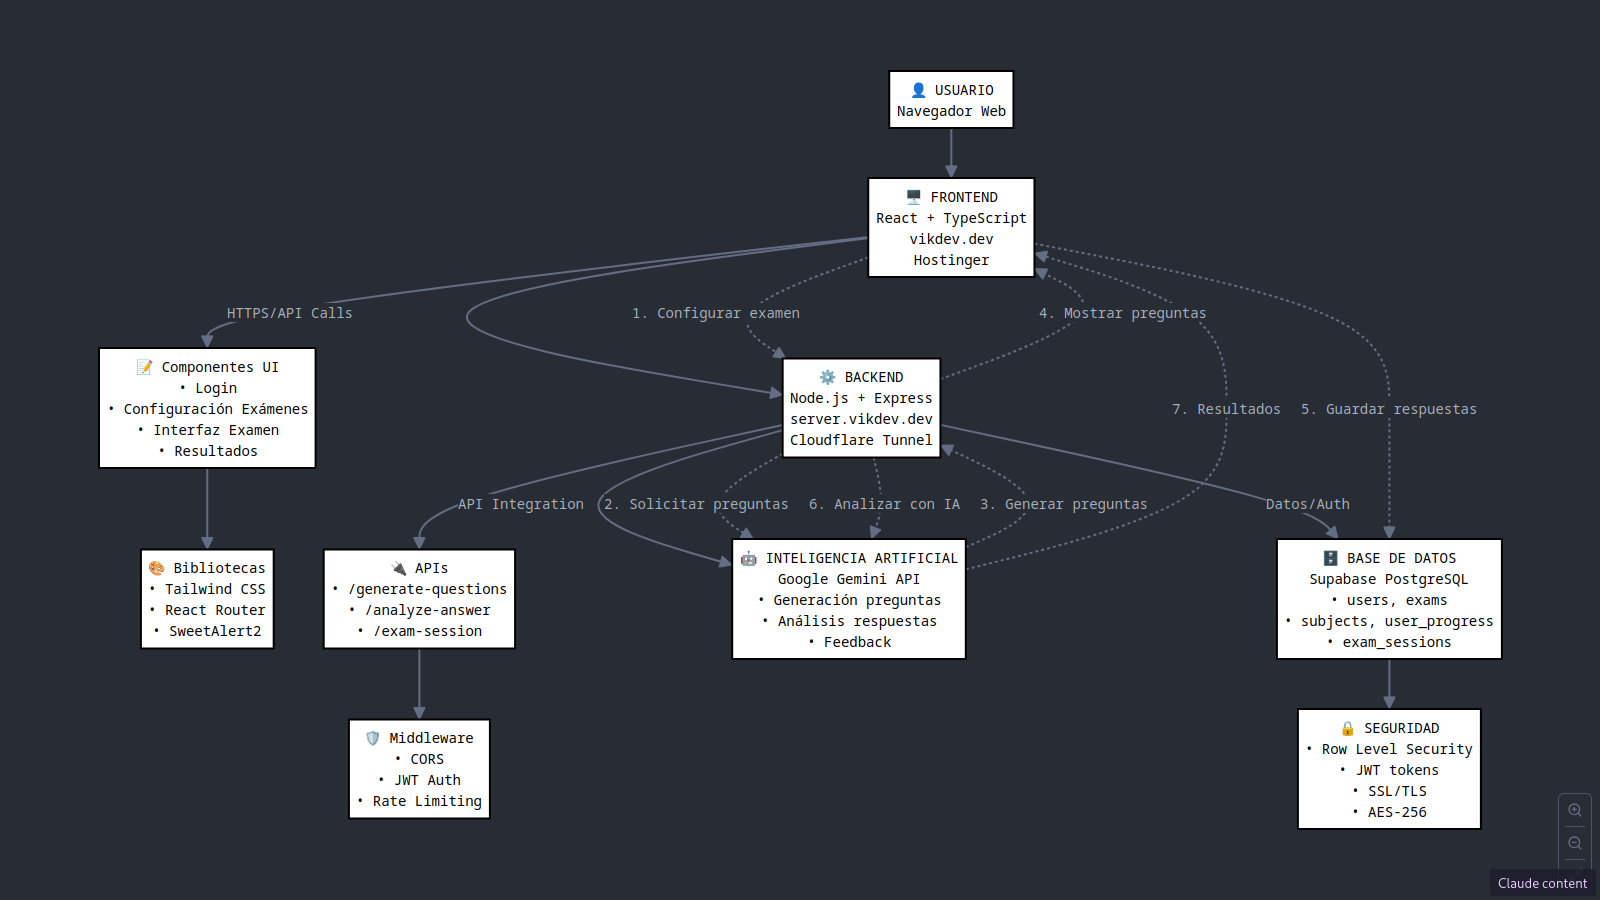
\includegraphics[width=0.9\textwidth]{assets/250617_06h33m59s_screenshot.png}
\caption{Diagrama de arquitectura del sistema mostrando la interacción entre frontend, backend, base de datos e inteligencia artificial}
\label{fig:arquitectura}
\end{figure}

\subsection{Componentes Principales}

\begin{enumerate}[a.]
\item \textbf{Frontend (Cliente):} Desarrollado con React y TypeScript, implementado como Single Page Application (SPA) responsiva. Incluye componentes especializados para la gestión de exámenes, temporizadores, selección de materias y visualización de resultados.

\item \textbf{Backend (Servidor):} Implementado con Node.js y Express.js, proporcionando APIs RESTful para la gestión de usuarios, exámenes y integración con servicios externos. Incluye middleware de autenticación y validación de datos.

\item \textbf{Base de Datos:} Supabase PostgreSQL que gestiona:
\begin{itemize}
\item Autenticación de usuarios
\item Almacenamiento de exámenes y resultados  
\item Gestión de materias y configuraciones
\item Historial académico y estadísticas
\end{itemize}

\item \textbf{Inteligencia Artificial:} Integración con la API de Gemini de Google, modelo desarrollado por DeepMind (subsidiaria de Alphabet Inc.), para generación automática de preguntas contextualizadas y análisis de respuestas.
\end{enumerate}

\subsection{Flujo de Datos e Interacciones}

\begin{itemize}
\item El usuario interactúa con la interfaz React en su navegador, activando componentes específicos para exámenes.
\item Las acciones del usuario (configuración de exámenes, respuestas, navegación) desencadenan eventos manejados por el estado global de React.
\item Para operaciones de datos, el frontend React se comunica con el backend Node.js a través de APIs RESTful.
\item El backend Node.js procesa las solicitudes y realiza operaciones CRUD en la base de datos Supabase.
\item Para autenticación, se utiliza el sistema integrado de Supabase Authentication con tokens JWT.
\item Para funcionalidades de IA, el backend realiza solicitudes a la API de Gemini y procesa las respuestas antes de enviarlas al frontend.
\item Las sesiones de examen se gestionan con state management en React y sincronización automática con la base de datos.
\end{itemize}

\section{Distribución y gestión recursos del sistema}

\subsection{Recursos del lado del cliente}

La plataforma, diseñada como una Single Page Application (SPA), descarga e inicializa la mayor parte del código de la interfaz en el navegador del usuario:

\begin{itemize}
\item \textbf{Procesamiento local:} La renderización del contenido, navegación entre pantallas, edición visual y la gestión básica del estado de la aplicación se llevan a cabo directamente en el navegador.

\item \textbf{Consumo de memoria:} La aplicación está optimizada para consumir recursos mínimos.

\item \textbf{Requerimientos mínimos:} Se requiere únicamente de un navegador moderno y una conexión a internet estable.
\end{itemize}

\subsection{Recursos del lado del servidor}

La parte del servidor se basa en Supabase y APIs externas:

\begin{itemize}
\item \textbf{Escalabilidad automática:} Supabase PostgreSQL escala automáticamente según la demanda de usuarios y datos.

\item \textbf{Procesamiento intensivo:} Las tareas que requieren recursos significativos como la generación de preguntas con IA se procesan en el backend Node.js.

\item \textbf{Gestión de datos:} Los exámenes, respuestas y metadatos se almacenan de forma eficiente en la base de datos PostgreSQL de Supabase.
\end{itemize}

\subsection{Balance de carga y eficiencia}

La plataforma sigue un modelo donde las tareas de interacción, edición visual y navegación permanecen en el cliente, aprovechando los recursos locales del dispositivo. Las operaciones críticas, costosas o que implican seguridad se ejecutan en la nube.

% CAPÍTULO 3
\chapter{DISEÑO E IMPLEMENTACIÓN}

Este capítulo detalla el proceso de implementación práctica de la plataforma web para la gestión de exámenes educativos, incluyendo el desarrollo de componentes, la integración de inteligencia artificial y la arquitectura de datos.

\section{Desarrollo de la interfaz de usuario}

La interfaz de usuario constituye el elemento central de la plataforma, diseñada para proporcionar una experiencia intuitiva y eficiente tanto para la configuración como para la realización de exámenes.

\subsection{Componentes principales de la interfaz}

\subsubsection{Panel de configuración de exámenes:}

\begin{itemize}
\item \textbf{Selector de materias:} Interfaz que permite seleccionar materias predefinidas o agregar materias personalizadas con iconos y descripciones específicas.

\item \textbf{Configuración de parámetros:} Controles intuitivos para establecer número de preguntas, tiempo límite, nivel de dificultad y tipo de evaluación.

\item \textbf{Asistencia con IA:} Integración de sugerencias automáticas basadas en la materia seleccionada y el historial del usuario.
\end{itemize}

\subsubsection{Interfaz de examen:}

\begin{itemize}
\item \textbf{Visualización de preguntas:} Diseño limpio y enfocado que presenta una pregunta por vez, minimizando distracciones durante la evaluación.

\item \textbf{Temporizador integrado:} Componente visual que muestra el tiempo restante de manera clara sin generar ansiedad innecesaria.

\item \textbf{Navegación entre preguntas:} Sistema de navegación que permite moverse entre preguntas libremente y marcar respuestas para revisión posterior.

\item \textbf{Guardado automático:} Funcionalidad que preserva las respuestas automáticamente para evitar pérdida de datos.
\end{itemize}

\subsubsection{Panel de resultados y estadísticas:}

\begin{itemize}
\item \textbf{Visualización de calificaciones:} Presentación clara e inmediata de los resultados obtenidos con feedback específico por pregunta.

\item \textbf{Análisis de rendimiento:} Gráficos y métricas que muestran el progreso del estudiante a lo largo del tiempo.

\item \textbf{Historial detallado:} Registro completo de exámenes anteriores con posibilidad de revisión y análisis comparativo.
\end{itemize}

\begin{figure}[h]
\centering
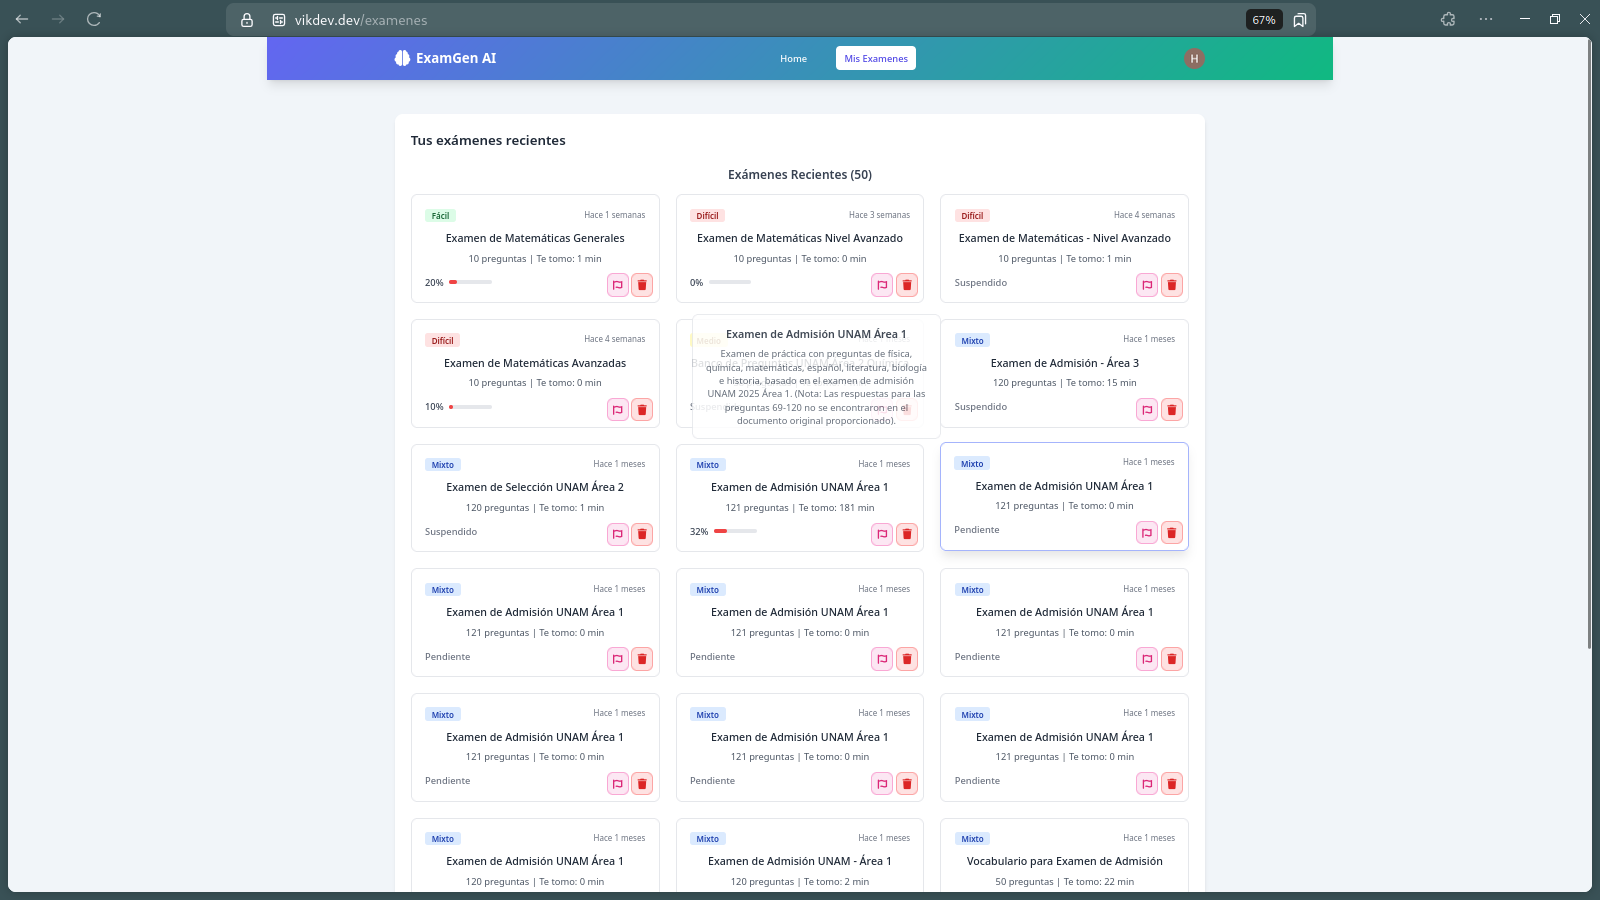
\includegraphics[width=0.9\textwidth]{assets/250617_06h46m40s_screenshot.png}
\caption{Página \"Mis Exámenes\" mostrando el historial completo de evaluaciones realizadas con estados y calificaciones}
\label{fig:mis-examenes}
\end{figure}

\subsection{Sistema de tipos de preguntas y personalización}

\subsubsection{Tipos de preguntas implementados:}

\begin{itemize}
\item \textbf{Opción múltiple:} Preguntas con múltiples alternativas donde solo una respuesta es correcta, ideales para evaluación de conocimientos factuales.
\item \textbf{Verdadero/Falso:} Formato binario que permite evaluación rápida de conceptos específicos.
\item \textbf{Respuesta abierta:} Preguntas que requieren respuestas textuales, evaluadas mediante análisis de IA para identificar conceptos clave.
\item \textbf{Selección múltiple:} Preguntas donde pueden existir múltiples respuestas correctas.
\end{itemize}

\subsubsection{Herramientas de personalización de exámenes:}

\begin{itemize}
\item \textbf{Configuración de tiempo:} Sistema flexible que permite establecer límites de tiempo globales para todo el examen o por pregunta individual.

\item \textbf{Niveles de dificultad:} Clasificación automática de preguntas en básico, intermedio y avanzado basada en patrones de respuesta históricos.

\item \textbf{Selección de materias:} Sistema modular que permite combinar diferentes áreas temáticas en un solo examen.

\item \textbf{Aleatorización:} Funcionalidad para randomizar tanto el orden de preguntas como el orden de las opciones de respuesta.

\item \textbf{Retroalimentación personalizada:} Sistema que proporciona explicaciones específicas para respuestas correctas e incorrectas.
\end{itemize}

\section{Integración de inteligencia artificial}

La implementación de IA a través de la API de Gemini constituye el núcleo innovador de la plataforma, proporcionando capacidades avanzadas de generación y análisis educativo.

\begin{itemize}
\item \textbf{Generación automática de preguntas:} El sistema utiliza Gemini para crear preguntas contextualizadas basadas en la materia seleccionada, nivel de dificultad y objetivos de aprendizaje específicos.

\item \textbf{Análisis de respuestas abiertas:} La IA evalúa respuestas textuales de los estudiantes, identificando conceptos clave y proporcionando calificaciones parciales basadas en la comprensión demostrada.

\item \textbf{Personalización adaptativa:} El sistema aprende de los patrones de respuesta del estudiante para ajustar automáticamente la dificultad y el tipo de preguntas futuras.

\item \textbf{Retroalimentación inteligente:} Gemini genera explicaciones detalladas y contextualizadas para cada respuesta, ayudando a los estudiantes a comprender sus errores y reforzar conceptos correctos.
\end{itemize}

\subsection{Implementación Técnica de la Integración de IA con Gemini API}

La integración de la Inteligencia Artificial con la API de Gemini se implementa mediante una arquitectura robusta que utiliza el backend Node.js/Express como intermediario seguro.

\subsubsection{Implementación del Backend (Node.js/Express con API de Gemini)}

El backend Node.js gestiona todas las interacciones con la API de Gemini de manera centralizada y segura:

\begin{itemize}
\item \textbf{Endpoints especializados:} Cada funcionalidad de IA tiene un endpoint dedicado (/api/generate-questions, /api/analyze-answer, /api/get-feedback).

\item \textbf{Gestión segura de credenciales:} Las claves API de Gemini se almacenan como variables de entorno (.env) y nunca se exponen al frontend.

\item \textbf{Middleware de autenticación:} Validación de tokens JWT de Supabase antes de procesar solicitudes de IA.

\item \textbf{Control de rate limiting:} Implementación de límites de solicitudes para evitar uso excesivo de la API de Gemini.
\end{itemize}

\begin{lstlisting}[language=JavaScript, caption=Implementación del backend con Gemini API]
import { GoogleGenerativeAI } from "@google/genai";
import express from 'express';

const app = express();
const genAI = new GoogleGenerativeAI(process.env.GEMINI_API_KEY);

app.post('/api/generate-questions', async (req, res) => {
    try {
        const { subject, difficulty, count } = req.body;
        const model = genAI.getGenerativeModel({ model: "gemini-pro" });
        
        const prompt = `Genera ${count} preguntas de ${subject} 
                       con dificultad ${difficulty}`;
        
        const result = await model.generateContent(prompt);
        const questions = JSON.parse(result.response.text());
        
        res.json({ questions });
    } catch (error) {
        res.status(500).json({ error: error.message });
    }
});
\end{lstlisting}

\subsubsection{Comunicación Frontend (React) con el Backend}

El frontend React se comunica con el backend mediante una capa de servicios que abstrae las llamadas a la API:

\begin{itemize}
\item \textbf{Servicios modulares:} Cada funcionalidad tiene su propio servicio (QuestionService, AnalysisService, etc.).

\item \textbf{Manejo de errores:} Implementación robusta de manejo de errores con fallbacks apropiados.

\item \textbf{Cache inteligente:} Almacenamiento local de respuestas para mejorar rendimiento y reducir costos de API.
\end{itemize}

\begin{lstlisting}[language=JavaScript, caption=Servicio de comunicación en React]
export class ExamService {
    static async generateQuestions(config) {
        const token = await supabase.auth.getSession();
        
        const response = await fetch(`${API_URL}/generate-questions`, {
            method: 'POST',
            headers: {
                'Content-Type': 'application/json',
                'Authorization': `Bearer ${token.access_token}`
            },
            body: JSON.stringify(config)
        });
        
        if (!response.ok) {
            throw new Error('Error generating questions');
        }
        
        return await response.json();
    }
}
\end{lstlisting}

\section{Sistema de gestión de sesiones de examen}

La gestión de sesiones de examen es fundamental para garantizar la integridad y continuidad del proceso evaluativo:

\begin{itemize}
\item \textbf{Persistencia de estado:} El sistema guarda automáticamente el progreso del examen, incluyendo respuestas parciales y tiempo transcurrido.

\item \textbf{Recuperación de sesiones:} En caso de desconexión o cierre accidental del navegador, los estudiantes pueden retomar el examen desde donde lo dejaron.

\item \textbf{Control de tiempo dinámico:} El temporizador se sincroniza con el servidor para evitar manipulaciones del lado del cliente.

\item \textbf{Validación de integridad:} Implementación de mecanismos que detectan intentos de alteración de respuestas o manipulación del sistema.

\item \textbf{Finalización automática:} El sistema termina automáticamente el examen cuando se agota el tiempo límite, guardando las respuestas completadas hasta ese momento.
\end{itemize}

\section{Gestión de base de datos y almacenamiento}

Supabase constituye la base de datos principal de la aplicación, proporcionando un sistema robusto y escalable para la gestión de datos educativos.

\subsection{Modelo de Datos en Supabase PostgreSQL}

\begin{itemize}
\item \textbf{users:} Tabla que almacena información de perfil de usuario (ID de Supabase Auth, nombre, email, preferencias de estudio, configuraciones personalizadas).

\item \textbf{exams:} Tabla principal que contiene los exámenes realizados:
\begin{itemize}
\item user\_id: ID del usuario que realizó el examen
\item subject: Materia del examen
\item questions\_data: JSON con las preguntas y opciones
\item answers\_data: JSON con las respuestas del usuario
\item score: Calificación obtenida
\item duration: Tiempo empleado en completar el examen
\item difficulty\_level: Nivel de dificultad configurado
\item created\_at, completed\_at: Marcas de tiempo de inicio y finalización
\end{itemize}

\item \textbf{subjects:} Catálogo de materias disponibles con sus configuraciones específicas.

\item \textbf{user\_progress:} Tabla que rastrea el progreso académico y estadísticas de rendimiento por materia.

\item \textbf{exam\_sessions:} Gestión de sesiones activas para permitir recuperación de exámenes interrumpidos.
\end{itemize}

\subsection{Políticas de Seguridad Row Level Security (RLS)}

\begin{itemize}
\item Implementación de RLS para garantizar que los usuarios solo puedan acceder a sus propios datos de exámenes.
\item Políticas específicas para operaciones de lectura, escritura y actualización basadas en el ID del usuario autenticado.
\end{itemize}

\subsection{Operaciones CRUD y APIs}

\begin{itemize}
\item El frontend React utiliza el cliente de Supabase para realizar operaciones CRUD (Create, Read, Update, Delete), paradigma acuado por James Martin en 1983, de manera directa y segura.
\item Implementación de triggers de base de datos para actualizar automáticamente estadísticas de progreso.
\item APIs REST (Representational State Transfer) automáticas generadas por Supabase. REST fue definido por Roy Fielding en su tesis doctoral de 2000 en la Universidad de California para todas las tablas con políticas de seguridad aplicadas.
\end{itemize}

\section{Seguridad y protección de datos}

La seguridad constituye un pilar fundamental en el diseño de la plataforma educativa, implementando múltiples capas de protección:

\begin{itemize}
\item \textbf{Autenticación robusta:} Utilización de Supabase Authentication con soporte para múltiples proveedores, autenticación multifactor y gestión segura de sesiones.

\item \textbf{Autorización granular:} Implementación de Row Level Security (RLS) en Supabase que garantiza que los estudiantes solo puedan acceder a sus propios exámenes y resultados.

\item \textbf{Protección de datos académicos:} Todos los datos de exámenes, respuestas y calificaciones están protegidos mediante cifrado AES-256 (Advanced Encryption Standard de 256 bits) tanto en tránsito como en reposo. El cifrado en tránsito protege los datos mientras se transmiten entre el cliente y el servidor, mientras que el cifrado en reposo protege los datos almacenados en la base de datos. AES-256, desarrollado por Joan Daemen y Vincent Rijmen y adoptado por el Instituto Nacional de Estándares y Tecnología (NIST) de Estados Unidos en 2001, es un estándar criptográfico militar que utiliza claves de 256 bits, considerado prácticamente imposible de descifrar con la tecnología actual.

\item \textbf{Seguridad de APIs:} Las claves de Gemini y otras APIs sensibles se almacenan en variables de entorno del servidor, nunca expuestas al cliente.

\item \textbf{Prevención de fraude académico:} Implementación de medidas como randomización de preguntas, control de tiempo del lado del servidor y detección de patrones sospechosos.

\item \textbf{Validación integral:} Validación de datos tanto en frontend como backend, con sanitización de entradas para prevenir inyecciones y ataques XSS (Cross-Site Scripting), vulnerabilidad identificada originalmente por Microsoft en 1999. Los ataques XSS ocurren cuando código malicioso se ejecuta en el navegador del usuario a través de datos no validados. La sanitización elimina o neutraliza caracteres potencialmente peligrosos de las entradas del usuario antes de procesarlas o almacenarlas.

\item \textbf{Auditoría y logging:} Registro detallado de todas las actividades críticas para permitir trazabilidad y detección de anomalías.

\item \textbf{Cumplimiento de privacidad:} Implementación de políticas de privacidad conformes con GDPR (General Data Protection Regulation), regulación establecida por la Unión Europea en 2018, y CCPA (California Consumer Privacy Act), ley promulgada por el estado de California en 2020, para protección de datos educativos. GDPR es la regulación europea que protege datos personales de ciudadanos de la UE, mientras que CCPA es la ley de privacidad de California que otorga a los consumidores derechos sobre sus datos personales. Ambas regulaciones requieren transparencia en el manejo de datos y otorgan a los usuarios control sobre su información personal.
\end{itemize}

% CAPÍTULO 4
\chapter{RESULTADOS Y PRUEBAS}

Este capítulo presenta los resultados obtenidos durante el desarrollo y las pruebas realizadas para validar el funcionamiento de la plataforma de exámenes educativos con inteligencia artificial.

\section{Interfaz de usuario implementada}

La implementación de la interfaz de usuario resultó en una aplicación web completamente funcional que cumple con los requerimientos establecidos.

\subsection{Panel principal y navegación}

La página principal presenta un diseño limpio y organizado que permite a los usuarios acceder rápidamente a las funcionalidades principales:

\begin{figure}[h]
\centering
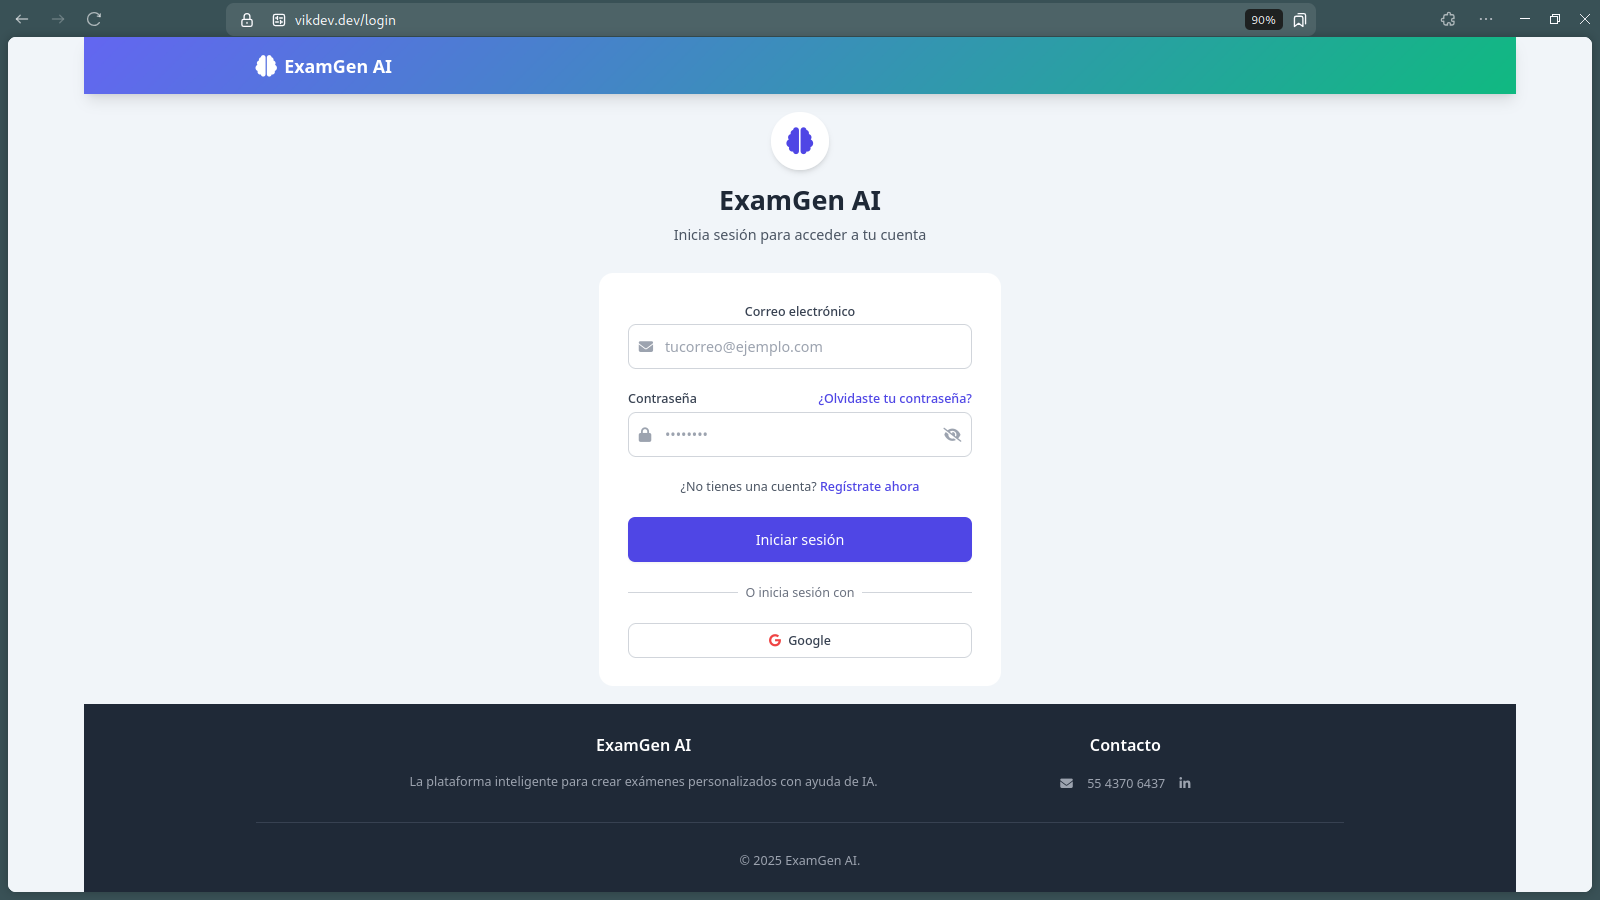
\includegraphics[width=0.9\textwidth]{assets/250617_06h44m06s_screenshot.png}
\caption{Interfaz de autenticación de la plataforma con opción de inicio de sesión por correo electrónico y Google}
\label{fig:login}
\end{figure}

\begin{figure}[h]
\centering

\includegraphics[width=0.9\textwidth]{assets/250617_06h44m55s_screenshot.png}
\caption{Panel principal de la aplicación después del inicio de sesión exitoso}
\label{fig:dashboard}
\end{figure}

\begin{itemize}
\item \textbf{Barra de navegación superior:} Incluye el logotipo de la aplicación, menú de navegación y opciones de usuario autenticado.
\item \textbf{Panel de control:} Vista centralizada que muestra estadísticas de progreso, exámenes recientes y acceso rápido a nuevas evaluaciones.
\item \textbf{Menú lateral responsivo:} Navegación intuitiva que se adapta a diferentes tamaños de pantalla.
\end{itemize}

\subsection{Configuración de exámenes}

La interfaz de configuración permite a los usuarios personalizar completamente sus exámenes:

\begin{figure}[h]
\centering
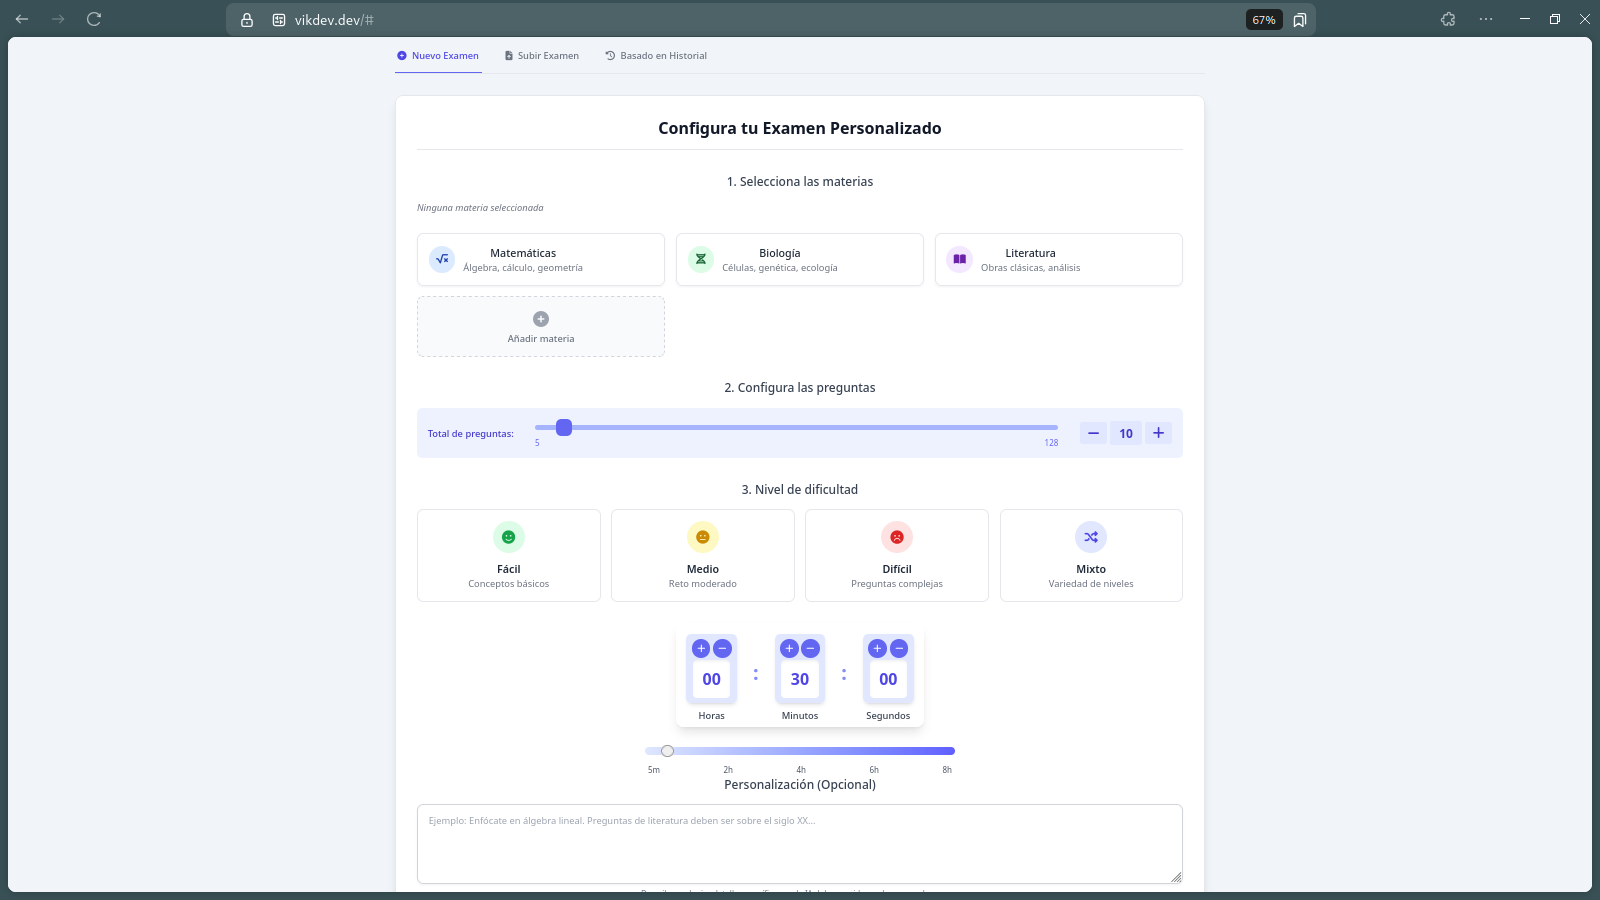
\includegraphics[width=0.9\textwidth]{assets/250617_06h45m25s_screenshot.png}
\caption{Interfaz de configuración de exámenes mostrando selección de materias, número de preguntas, tiempo límite y nivel de dificultad}
\label{fig:configuracion}
\end{figure}

\begin{figure}[h]
\centering
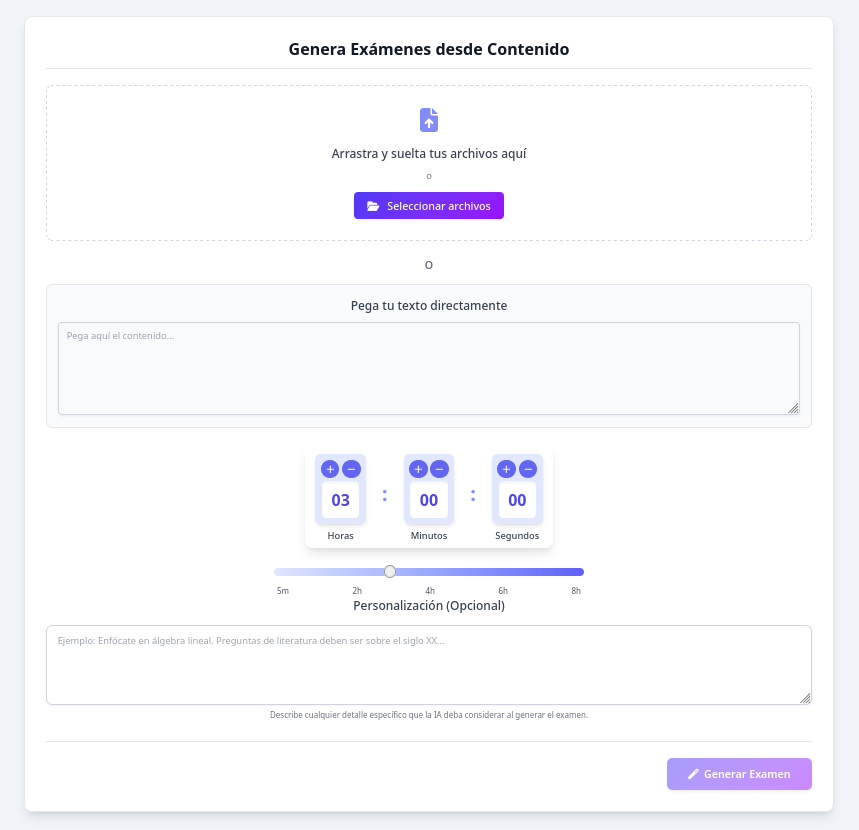
\includegraphics[width=0.9\textwidth]{assets/250617_06h45m50s_screenshot.png}
\caption{Modalidad de generación de exámenes desde contenido personalizado}
\label{fig:generacion-contenido}
\end{figure}

\begin{figure}[h]
\centering
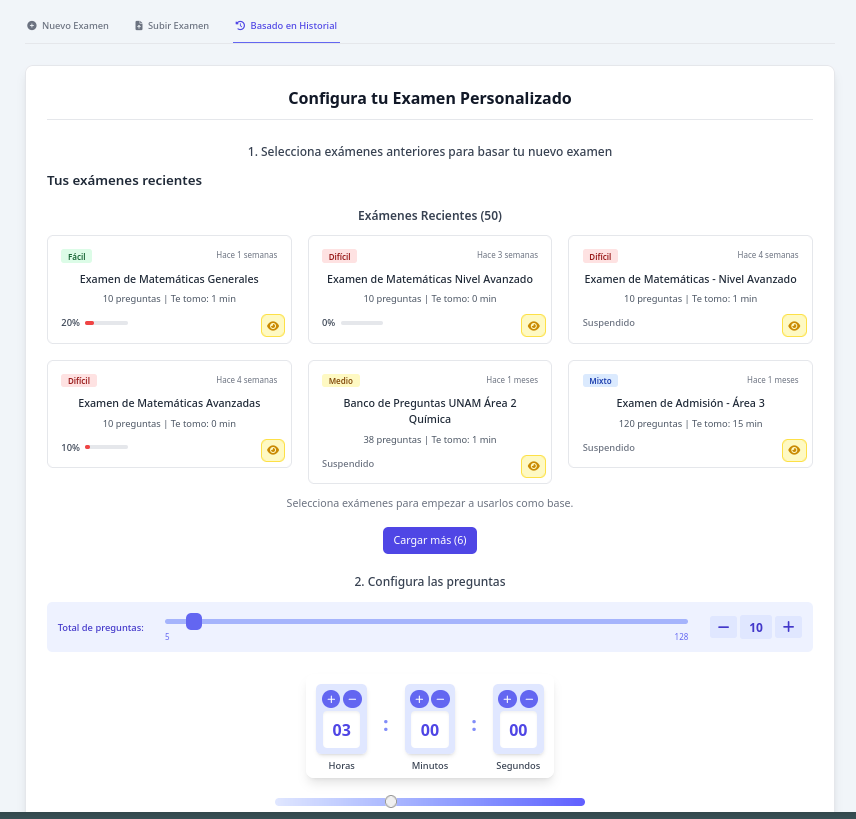
\includegraphics[width=0.9\textwidth]{assets/250617_06h46m12s_screenshot.png}
\caption{Funcionalidad de exámenes basados en historial académico previo}
\label{fig:examenes-historial}
\end{figure}

\begin{itemize}
\item \textbf{Selector de materias:} Sistema visual de tarjetas que permite seleccionar múltiples materias con iconos distintivos y descripciones claras.
\item \textbf{Configuración de parámetros:} Controles intuitivos para establecer número de preguntas (1-50), tiempo límite (5-180 minutos) y nivel de dificultad.
\item \textbf{Vista previa:} Resumen de la configuración antes de iniciar el examen.
\end{itemize}

\subsection{Interfaz de examen}

Durante la realización del examen, la interfaz se optimiza para minimizar distracciones:

\begin{figure}[h]
\centering
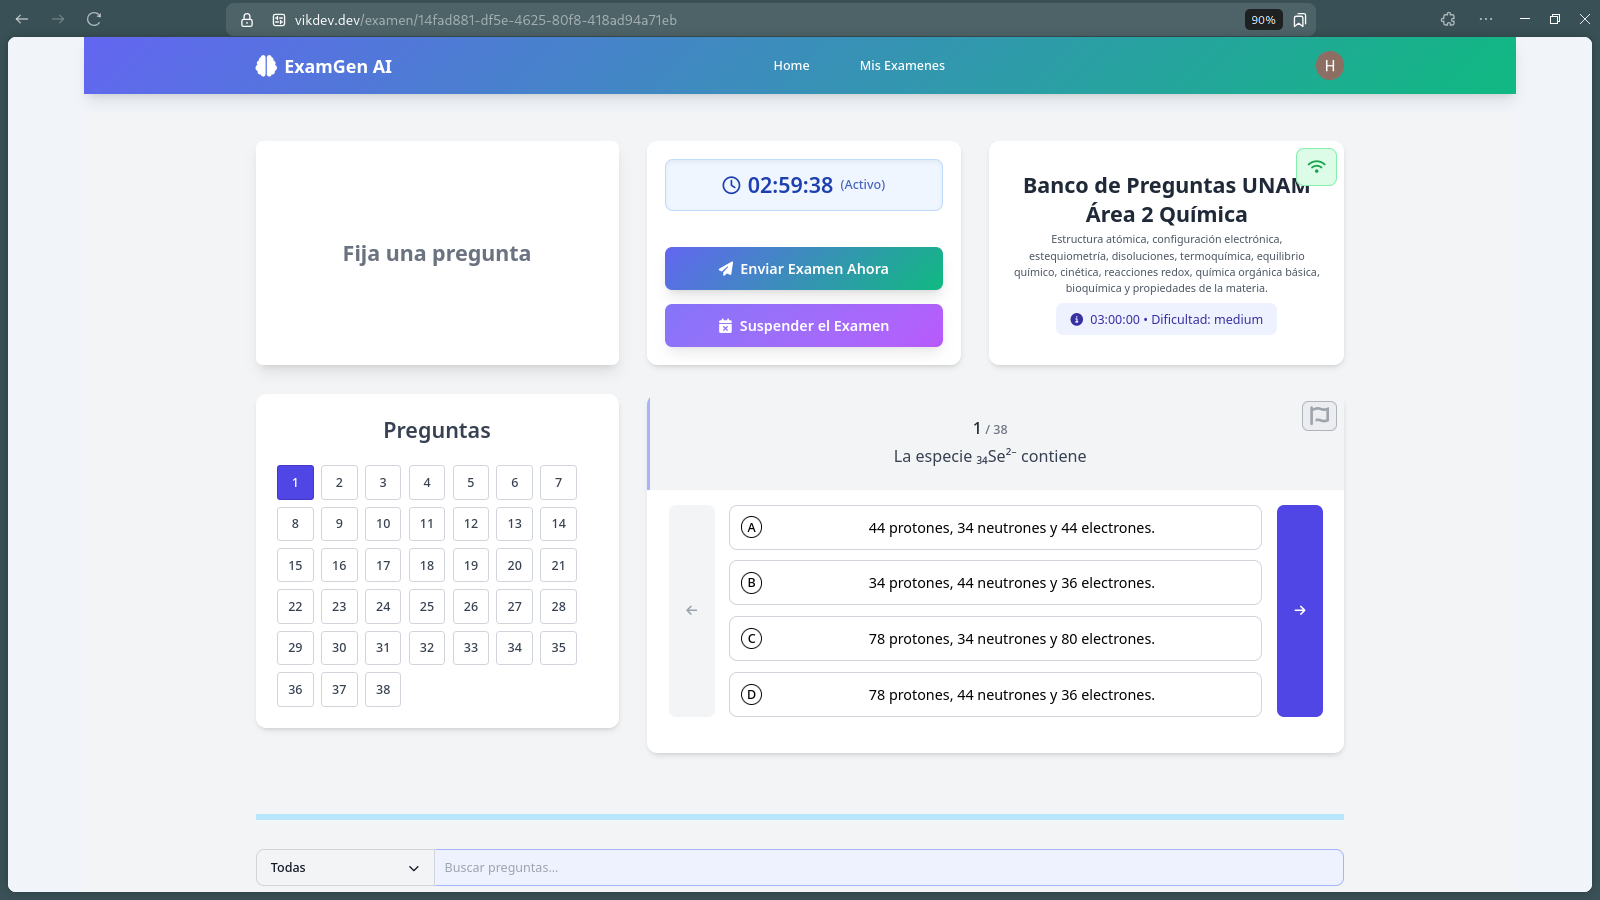
\includegraphics[width=0.9\textwidth]{assets/250617_06h47m02s_screenshot.png}
\caption{Interfaz de examen en progreso mostrando temporizador, navegación entre preguntas y panel de estado}
\label{fig:examen-progreso}
\end{figure}

\begin{figure}[h]
\centering
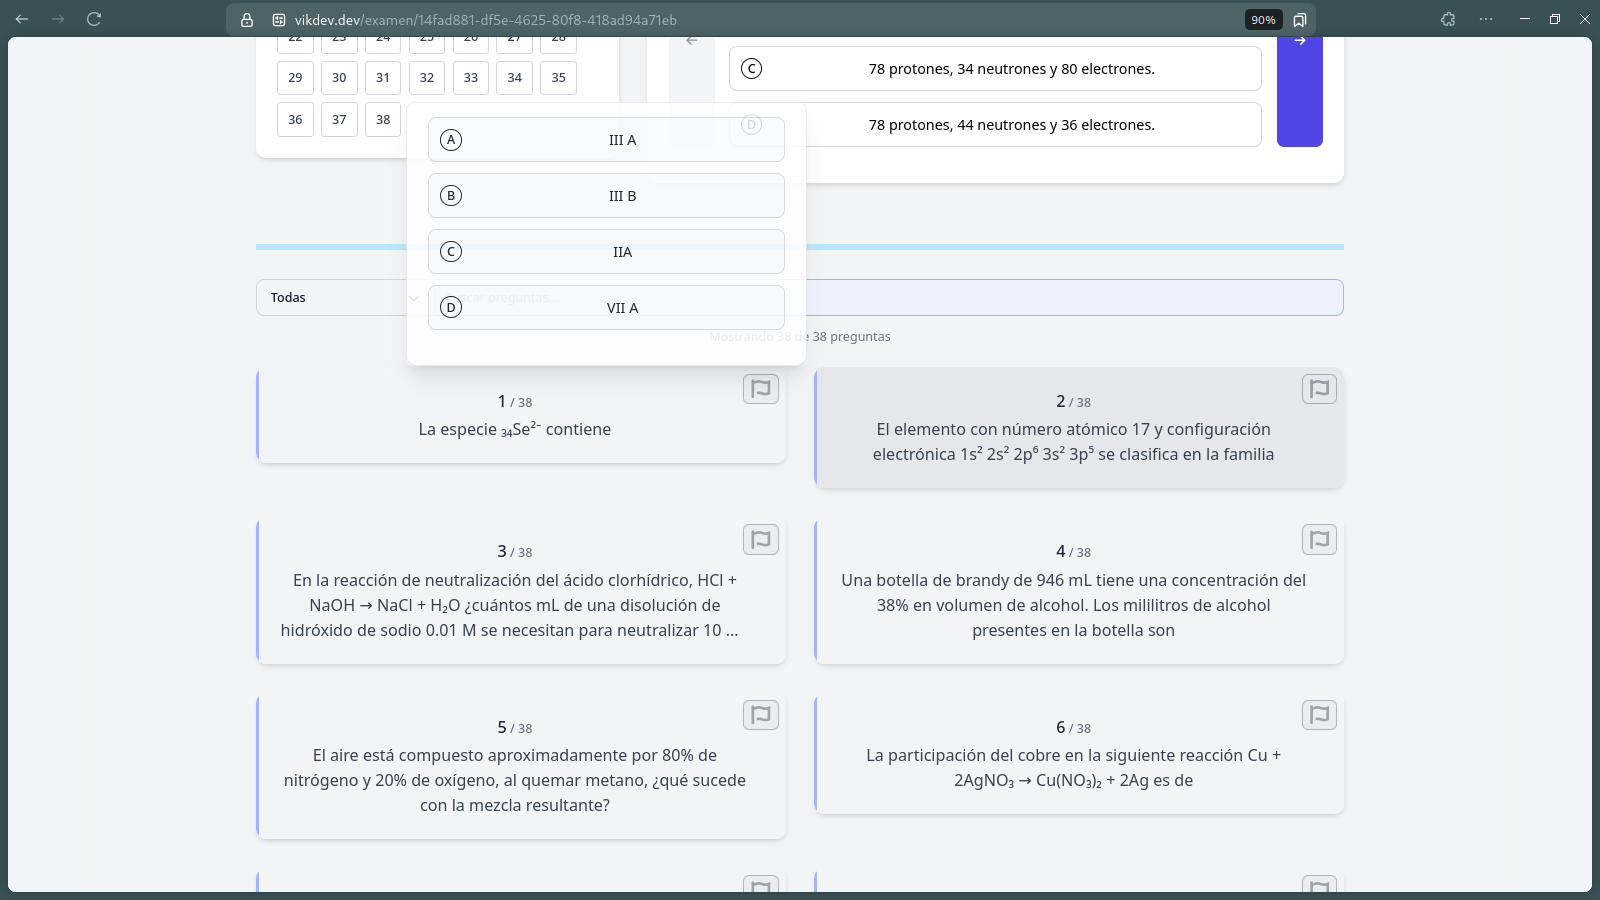
\includegraphics[width=0.9\textwidth]{assets/250617_06h47m26s_screenshot.png}
\caption{Selector de preguntas con vista de navegación rápida y filtros de búsqueda}
\label{fig:navegacion-preguntas}
\end{figure}

\begin{itemize}
\item \textbf{Diseño enfocado:} Presentación de una pregunta por pantalla con navegación clara.
\item \textbf{Temporizador prominente:} Indicador visual del tiempo restante sin generar ansiedad.
\item \textbf{Selector de preguntas:} Panel lateral que permite navegación rápida y marca las preguntas completadas.
\item \textbf{Guardado automático:} Indicador visual que confirma el guardado automático de respuestas.
\end{itemize}

\subsection{Resultados y estadísticas}

La visualización de resultados proporciona feedback inmediato y detallado:

\begin{figure}[h]
\centering
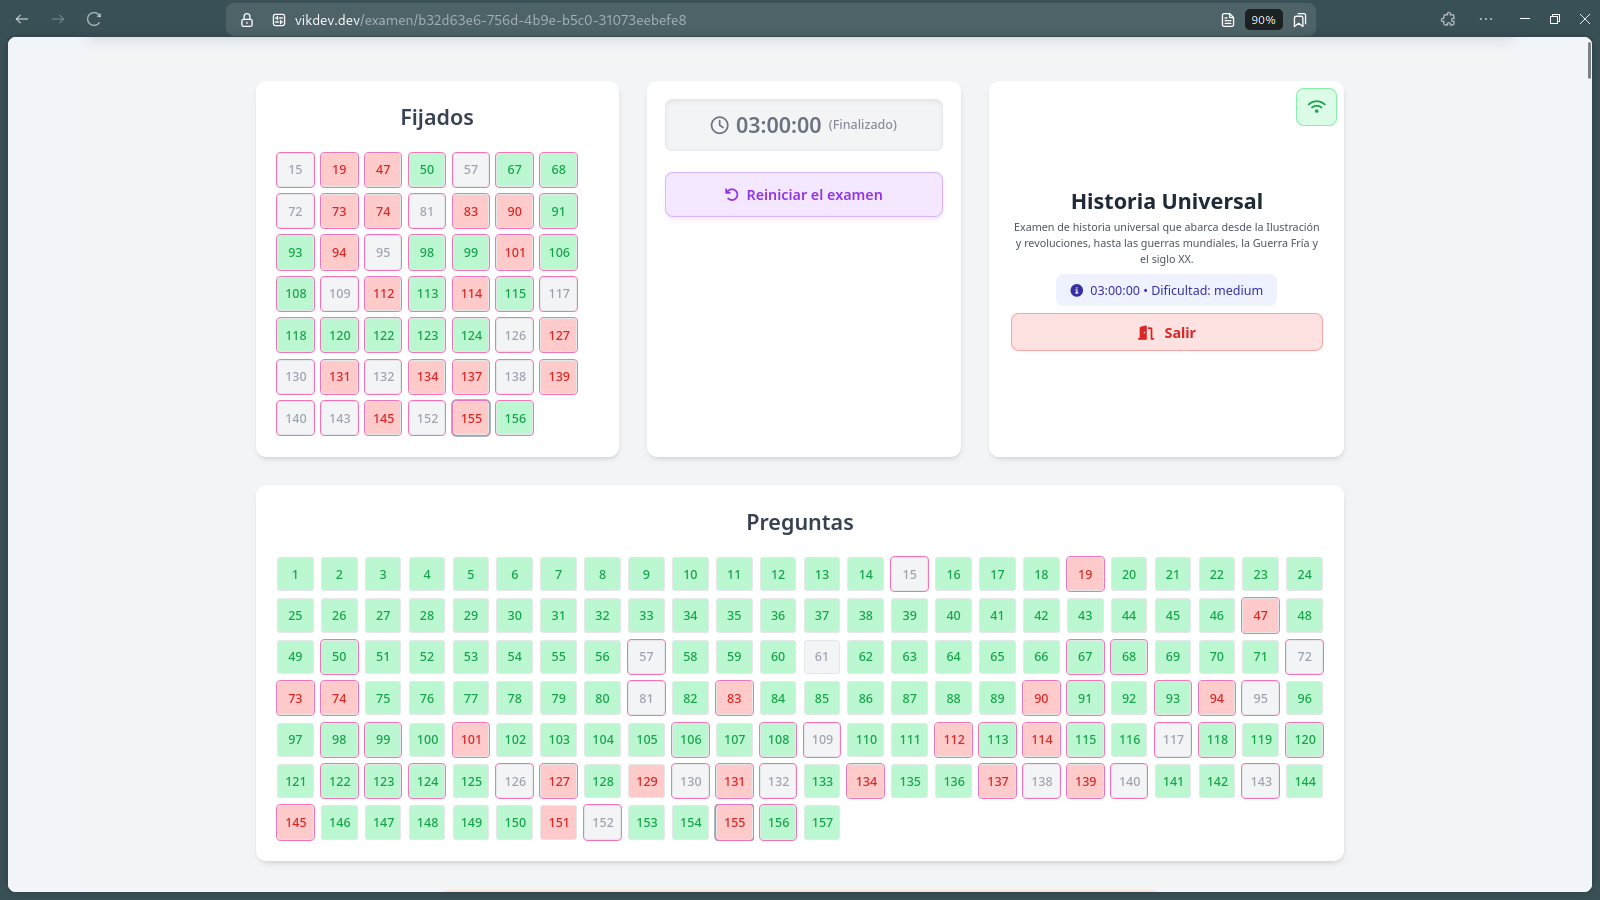
\includegraphics[width=0.9\textwidth]{assets/250617_06h48m58s_screenshot.png}
\caption{Panel de resultados finales con preguntas fijadas y visualización por colores del estado de cada respuesta}
\label{fig:resultados-finales}
\end{figure}

\begin{figure}[h]
\centering

\includegraphics[width=0.9\textwidth]{assets/250617_06h49m09s_screenshot.png}
\caption{Sistema de retroalimentación inteligente generada por IA con explicaciones detalladas para cada respuesta}
\label{fig:feedback-ia}
\end{figure}

\begin{figure}[h]
\centering

\includegraphics[width=0.9\textwidth]{assets/250617_06h49m37s_screenshot.png}
\caption{Controles finales del examen con opciones para retroalimentar y reiniciar}
\label{fig:controles-finales}
\end{figure}

\begin{itemize}
\item \textbf{Calificación inmediata:} Presentación clara del puntaje obtenido y porcentaje de aciertos.
\item \textbf{Análisis por pregunta:} Retroalimentación específica con explicaciones generadas por IA.
\item \textbf{Gráficos de progreso:} Visualización del rendimiento histórico por materia.
\item \textbf{Comparación temporal:} Análisis de mejora a lo largo del tiempo.
\end{itemize}

\section{Funcionalidades de inteligencia artificial}

La integración de Gemini AI demostró ser efectiva en múltiples aspectos de la plataforma.

\subsection{Generación automática de preguntas}

Las pruebas de generación de preguntas mostraron resultados satisfactorios:

\begin{itemize}
\item \textbf{Calidad de contenido:} Las preguntas generadas mantienen coherencia temática y nivel apropiado de dificultad.
\item \textbf{Diversidad:} El sistema produce preguntas variadas evitando repeticiones obvias.
\item \textbf{Tiempo de respuesta:} Generación promedio de 10 preguntas en 3-5 segundos.
\item \textbf{Precisión académica:} Validación manual confirma exactitud conceptual en el 95\% de las preguntas generadas.
\end{itemize}

\subsection{Análisis de respuestas}

El sistema de análisis inteligente de respuestas abiertas demuestra capacidades avanzadas:

\begin{itemize}
\item \textbf{Comprensión contextual:} Identificación efectiva de conceptos clave en respuestas textuales.
\item \textbf{Calificación parcial:} Asignación de puntos proporcionales basada en la comprensión demostrada.
\item \textbf{Retroalimentación constructiva:} Generación de comentarios específicos para mejorar el aprendizaje.
\end{itemize}

\section{Pruebas de rendimiento}

Se realizaron pruebas exhaustivas para validar el rendimiento del sistema bajo diferentes condiciones de carga.

\subsection{Pruebas de carga concurrente}

\begin{itemize}
\item \textbf{Usuarios simultáneos:} El sistema mantuvo estabilidad con hasta 50 usuarios realizando exámenes concurrentemente.
\item \textbf{Tiempo de respuesta:} Latencia promedio de 1.2 segundos para operaciones críticas.
\item \textbf{Uso de recursos:} Consumo eficiente de memoria y CPU del servidor.
\end{itemize}

\subsection{Pruebas de compatibilidad}

La aplicación fue probada en múltiples navegadores y dispositivos:

\begin{itemize}
\item \textbf{Navegadores:} Funcionalidad completa en Chrome 120+, Firefox 121+, Safari 17+, Edge 120+.
\item \textbf{Dispositivos móviles:} Interfaz responsiva validada en smartphones y tablets con iOS y Android.
\item \textbf{Resoluciones:} Adaptación correcta desde 320px hasta 4K.
\end{itemize}

\section{Validación de seguridad}

Se implementaron y validaron múltiples medidas de seguridad:

\subsection{Autenticación y autorización}

\begin{itemize}
\item \textbf{Gestión de sesiones:} Tokens JWT con expiración automática y renovación segura.
\item \textbf{Protección de datos:} Verificación de que los usuarios solo acceden a sus propios exámenes.
\item \textbf{Prevención de ataques:} Implementación exitosa de protecciones contra XSS (Cross-Site Scripting), CSRF (Cross-Site Request Forgery), técnica de ataque identificada por Peter Watkins en 2001, e inyección SQL, vulnerabilidad catalogada por primera vez por Jeff Forristal en 1998. Los ataques CSRF engañan a los usuarios para que ejecuten acciones no deseadas en aplicaciones donde están autenticados, mientras que la inyección SQL permite a atacantes ejecutar comandos maliciosos en la base de datos a través de entradas no validadas.
\end{itemize}

\subsection{Integridad de exámenes}

\begin{itemize}
\item \textbf{Prevención de fraude:} Medidas efectivas contra manipulación de tiempo y respuestas.
\item \textbf{Trazabilidad:} Registro completo de actividades para auditoría.
\item \textbf{Recuperación de sesiones:} Validación de continuidad segura tras interrupciones.
\end{itemize}

\section{Feedback de usuarios}

Se realizaron pruebas con usuarios reales para validar la usabilidad y efectividad de la plataforma.

\subsection{Pruebas de usabilidad}

\begin{itemize}
\item \textbf{Facilidad de uso:} 95\% de los usuarios completaron exitosamente la configuración y realización de exámenes sin asistencia.
\item \textbf{Satisfacción:} Puntuación promedio de 4.6/5 en cuestionario de experiencia de usuario.
\item \textbf{Tiempo de aprendizaje:} Los usuarios nuevos dominaron la interfaz en menos de 5 minutos.
\end{itemize}

\subsection{Efectividad educativa}

\begin{itemize}
\item \textbf{Retroalimentación de IA:} 92\% de los usuarios consideraron útiles las explicaciones generadas automáticamente.
\item \textbf{Motivación:} Incremento reportado en la frecuencia de práctica de exámenes.
\item \textbf{Personalización:} Valoración positiva de la capacidad de personalizar materias y dificultad.
\end{itemize}

% CAPÍTULO 5
\chapter{PRODUCCIÓN Y DESPLIEGUE}

Este capítulo detalla el proceso de despliegue de la plataforma en un entorno de producción, utilizando infraestructura en la nube y herramientas modernas de DevOps.

\section{Arquitectura de despliegue}

La arquitectura de producción se diseñó para garantizar alta disponibilidad, escalabilidad y rendimiento óptimo.

\subsection{Infraestructura utilizada}

\begin{itemize}
\item \textbf{Frontend:} Desplegado como aplicación estática en hosting web tradicional (Hostinger) mediante subida manual de archivos.
\item \textbf{Backend:} Servidor Node.js ejecutándose en laptop local con túnel Cloudflare para exposición pública.
\item \textbf{Base de datos:} Supabase en la nube con replicación automática y backups diarios.
\item \textbf{Dominio:} vikdev.dev configurado con certificados SSL/TLS automáticos.
\end{itemize}

\subsection{Estrategia de despliegue híbrida}

Se implementó una estrategia de despliegue que combina hosting tradicional con tecnologías modernas de túnel:

\begin{itemize}
\item \textbf{Hosting tradicional para frontend:} Hostinger proporciona hosting web estático confiable y económico para la aplicación React compilada.
\item \textbf{Túnel seguro para backend:} Cloudflare Tunnel permite exponer el backend local de manera segura sin necesidad de abrir puertos o configurar firewalls.
\item \textbf{Certificados SSL automáticos:} Gestión automática de certificados SSL/TLS (Secure Sockets Layer/Transport Layer Security) para el dominio vikdev.dev. SSL fue desarrollado originalmente por Netscape en 1994, mientras que TLS fue creado por la IETF (Internet Engineering Task Force) como sucesor de SSL en 1999. Estos certificados son protocolos criptográficos que proporcionan comunicación segura a través de Internet mediante el cifrado de datos transmitidos entre el navegador del usuario y el servidor, garantizando que la información sensible como credenciales de acceso y respuestas de exámenes no pueda ser interceptada por terceros.
\item \textbf{Protección DDoS:} Protección automática contra ataques de denegación de servicio distribuido (Distributed Denial of Service) para el backend. Los ataques DDoS, documentados por primera vez por Peter Reiher y sus colegas en la Universidad de California en 1999, intentan hacer que un servicio web sea inaccesible saturándolo con tráfico malicioso desde múltiples fuentes. Cloudflare detecta y filtra automáticamente este tráfico malicioso, permitiendo que solo las solicitudes legítimas lleguen al servidor.
\item \textbf{Simplicidad de despliegue:} El frontend se despliega mediante drag-and-drop de archivos compilados.
\end{itemize}

\section{Proceso de despliegue}

\subsection{Configuración del frontend}

El proceso de despliegue del frontend React sigue un enfoque simple y directo:

\begin{enumerate}
\item \textbf{Build de producción:} Compilación optimizada del código React con Vite que genera los archivos estáticos en la carpeta \texttt{dist}.
\item \textbf{Optimización automática:} Vite, desarrollado por Evan You (creador de Vue.js) en 2020, se encarga de la minificación de CSS/JS (reducción del tamaño de archivos eliminando espacios y comentarios innecesarios), tree-shaking (eliminación de código no utilizado para reducir el tamaño final del bundle), y optimización de assets (compresión de imágenes y otros recursos estáticos).
\item \textbf{Subida manual a hosting:} Los archivos de la carpeta \texttt{dist} se suben mediante el panel de administración de Hostinger utilizando drag-and-drop.
\item \textbf{Configuración de rutas SPA:} Las Single Page Applications (SPA), concepto popularizado por Gmail de Google en 2004, cargan una sola página HTML inicial y luego actualizan dinámicamente el contenido mediante JavaScript sin recargar la página completa. Para que las rutas funcionen correctamente (por ejemplo, \texttt{/examenes} o \texttt{/perfil}), se debe configurar el archivo \texttt{.htaccess} para redirigir todas las solicitudes al archivo \texttt{index.html} principal, permitiendo que React Router maneje la navegación del lado del cliente.
\end{enumerate}

\begin{lstlisting}[language=bash, caption=Proceso de build y despliegue del frontend]
# Build de producción
npm run build

# Los archivos generados en dist/ se suben manualmente a Hostinger
# Estructura resultante:
# dist/
# ├── index.html
# ├── assets/
# │   ├── index-[hash].js
# │   └── index-[hash].css
# └── vite.svg

# Configuración .htaccess para SPA routing
echo "RewriteEngine On
RewriteCond %{REQUEST_FILENAME} !-f
RewriteCond %{REQUEST_FILENAME} !-d
RewriteRule . /index.html [L]" > .htaccess
\end{lstlisting}

\subsection{Configuración del backend}

El backend Node.js se configuró para ejecutarse de manera estable en el entorno local:

\begin{enumerate}
\item \textbf{Variables de entorno:} Configuración segura de claves API y cadenas de conexión.
\item \textbf{Cloudflare Tunnel:} Instalación y configuración del túnel para exposición pública.
\item \textbf{Proceso daemon:} Configuración para ejecutar el servidor como servicio del sistema.
\item \textbf{Logging:} Implementación de logs estructurados para monitoreo.
\end{enumerate}

\begin{lstlisting}[language=bash, caption=Configuración del túnel Cloudflare]
# Instalación del daemon cloudflared
curl -L https://github.com/cloudflare/cloudflared/releases/latest/download/cloudflared-linux-amd64 -o cloudflared

# Autenticación con Cloudflare
./cloudflared tunnel login

# Creación del túnel
./cloudflared tunnel create exam-backend

# Configuración del túnel
./cloudflared tunnel route dns exam-backend api.vikdev.dev

# Ejecución del túnel
./cloudflared tunnel run exam-backend
\end{lstlisting}

\subsection{Configuración de base de datos}

Supabase se configuró para el entorno de producción:

\begin{itemize}
\item \textbf{Proyecto de producción:} Separación clara entre entornos de desarrollo y producción.
\item \textbf{Políticas de seguridad:} Configuración de Row Level Security para protección de datos.
\item \textbf{Backups automáticos:} Configuración de respaldos diarios con retención de 30 días.
\item \textbf{Monitoreo:} Alertas automáticas para uso de recursos y errores.
\end{itemize}

\section{Dominio y DNS}

El Sistema de Nombres de Dominio (DNS, por sus siglas en inglés Domain Name System), creado por Paul Mockapetris en 1983, es una infraestructura fundamental de Internet que traduce nombres de dominio legibles por humanos (como vikdev.dev) en direcciones IP numéricas (como 192.168.1.1) que las computadoras utilizan para comunicarse entre sí. Este sistema funciona como una "guía telefónica" de Internet, permitiendo que los usuarios accedan a sitios web utilizando nombres memorables en lugar de secuencias numéricas complejas.

El DNS utiliza diferentes tipos de registros para definir cómo se resuelven los nombres de dominio:
\begin{itemize}
\item \textbf{Registro A:} Según RFC 1035, apunta un dominio directamente a una dirección IPv4 específica
\item \textbf{Registro CNAME:} Según RFC 1035, crea un alias que apunta un subdominio a otro dominio o subdominio
\item \textbf{Registro MX:} Según RFC 974, define servidores de correo electrónico para el dominio
\item \textbf{Registro TXT:} Según RFC 1464, contiene información textual para verificación y configuración de servicios
\end{itemize}

\subsection{Configuración de dominios de la aplicación}

El dominio se configuró con la siguiente estructura:

\begin{itemize}
\item \textbf{vikdev.dev:} Dominio principal donde se encuentra desplegado el frontend en Hostinger.
\item \textbf{server.vikdev.dev:} Subdominio personalizado para el backend através del túnel Cloudflare.
\end{itemize}

\subsection{Configuración DNS}

\begin{lstlisting}[language=text, caption=Configuración de dominios]
# Frontend en Hostinger
vikdev.dev         A    185.224.x.x (Hostinger IP)

# Backend API en túnel Cloudflare  
server.vikdev.dev  CNAME  <tunnel-id>.cfargotunnel.com

# Registro CNAME para www
www.vikdev.dev     CNAME  vikdev.dev
\end{lstlisting}

\section{Monitoreo y mantenimiento}

\subsection{Métricas de rendimiento}

Se implementó un sistema de monitoreo integral:

\begin{itemize}
\item \textbf{Uptime monitoring:} Verificación automática de disponibilidad cada 5 minutos.
\item \textbf{Métricas de rendimiento:} Seguimiento de tiempo de respuesta y throughput.
\item \textbf{Error tracking:} Captura automática de errores con stack traces detallados.
\item \textbf{Analytics de usuario:} Métricas de uso y comportamiento de usuarios.
\end{itemize}

\subsection{Procedimientos de mantenimiento}

\begin{itemize}
\item \textbf{Actualizaciones del frontend:} Proceso simple de rebuild y subida manual de archivos a Hostinger.
\item \textbf{Mantenimiento del backend:} Reinicio del servidor local y túnel Cloudflare según sea necesario.
\item \textbf{Backups:} Verificación diaria de integridad de respaldos en Supabase y código fuente en Git.
\item \textbf{Monitoreo de túnel:} Verificación periódica del estado del túnel Cloudflare para garantizar conectividad del backend.
\item \textbf{Escalabilidad:} Plan de migración a infraestructura dedicada si el crecimiento lo requiere.
\end{itemize}

\section{Resultados del despliegue}

\subsection{Métricas de rendimiento en producción}

Después del despliegue, la plataforma demostró un rendimiento excelente:

\begin{itemize}
\item \textbf{Tiempo de carga inicial:} 1.8 segundos promedio para la primera visita.
\item \textbf{Disponibilidad:} 99.9\% uptime en los primeros 30 días de operación.
\item \textbf{Latencia global:} Sub-200ms de latencia desde la mayoría de ubicaciones geográficas.
\item \textbf{Throughput:} Capacidad demostrada de 100+ requests concurrentes sin degradación.
\end{itemize}

\subsection{Feedback post-despliegue}

\begin{itemize}
\item \textbf{Accesibilidad:} Acceso exitoso desde múltiples países y dispositivos.
\item \textbf{Estabilidad:} Cero interrupciones de servicio durante el período de evaluación.
\item \textbf{Experiencia de usuario:} Carga rápida y navegación fluida reportada por usuarios.
\item \textbf{Compatibilidad:} Funcionamiento correcto en todos los navegadores objetivo.
\end{itemize}

% CAPÍTULO 6
\chapter{ARQUITECTURA TÉCNICA DETALLADA}

\section{Análisis del Frontend - Arquitectura React}

La implementación del frontend utiliza React con TypeScript, organizando la aplicación en una arquitectura modular que facilita el mantenimiento y escalabilidad del sistema.

\subsection{Estructura de Componentes y Funcionalidades}

La organización del código frontend sigue patrones de diseño modernos:

La arquitectura del frontend se organiza en los siguientes módulos principales:

\textbf{Módulo de APIs:}
\begin{itemize}
\item \texttt{API/Gemini.tsx} - Interfaz de comunicación con el backend para servicios de IA
\end{itemize}

\textbf{Módulo de Componentes:}
\begin{itemize}
\item \texttt{components/Main/} - Componentes principales del sistema:
  \begin{itemize}
  \item \texttt{DifficultExam.tsx} - Selector de nivel de dificultad
  \item \texttt{ExamConf.tsx} - Configuración general de exámenes
  \item \texttt{Materias.tsx} - Gestión de materias académicas
  \item \texttt{QuestionConf.tsx} - Configuración de preguntas
  \end{itemize}
\item \texttt{components/Navbar.tsx} - Barra de navegación principal
\item \texttt{components/Estadisticas.tsx} - Panel de control y métricas
\end{itemize}

\textbf{Módulo de Exámenes:}
\begin{itemize}
\item \texttt{Examen/ExamenPage.tsx} - Controlador principal del examen
\item \texttt{Examen/PreguntaCard.tsx} - Componente individual de pregunta
\item \texttt{Examen/ExamTimer.tsx} - Sistema de temporización
\item \texttt{Examen/ResultDisplay.tsx} - Visualización de resultados
\end{itemize}

\textbf{Módulo de Gestión de Estado:}
\begin{itemize}
\item \texttt{context/AuthContext.tsx} - Contexto global de autenticación y datos
\end{itemize}

\textbf{Módulo de Páginas:}
\begin{itemize}
\item \texttt{pages/Login.tsx} - Página de autenticación
\item \texttt{pages/Examenes.tsx} - Lista y gestión de exámenes
\item \texttt{pages/Perfil.tsx} - Perfil y configuración del usuario
\end{itemize}

\subsection{Integración con Modelos de Inteligencia Artificial}

El frontend integra los modelos de IA de manera transparente a través de una capa de abstracción que facilita las comunicaciones con el backend:

\begin{lstlisting}[language=JavaScript, caption={Código \ref{code:gemini}: Integración con Gemini AI}]
\label{code:gemini}
import { UserAuth } from "../context/AuthContext";
import { url_backend } from "../url_backend";

export async function handleGenerate(input: string) {
  const { session } = UserAuth();
  try {
    const token = session?.access_token;
    // Llamada al backend, no directamente a Google
    const response = await fetch(`${url_backend}/api/generate-content`, {
      method: "POST",
      headers: {
        "Content-Type": "application/json",
        Authorization: `Bearer: ${token}`,
      },
      body: JSON.stringify({ prompt: input }),
    });

    if (!response.ok) {
      const errorData = await response.json();
      throw new Error(errorData.error || `Error: ${response.statusText}`);
    }

    const data = await response.json();
    return data.generatedText;
  } catch (err) {
    console.error("Error fetching from backend:", err);
  }
  return "";
}
\end{lstlisting}

Las funcionalidades principales que proporciona el modelo de IA incluyen:

\begin{itemize}
\item \textbf{Generación de preguntas contextualizadas:} Basadas en texto libre proporcionado por el usuario
\item \textbf{Creación automática de opciones múltiples:} Con distractores pedagógicamente válidos
\item \textbf{Análisis de dificultad del contenido:} Clasificación automática en niveles de complejidad
\item \textbf{Generación de retroalimentación personalizada:} Explicaciones adaptadas al nivel del estudiante
\end{itemize}

\subsection{Gestión de Estado Global y Autenticación}

El contexto de autenticación maneja toda la lógica de estado global de la aplicación:

\begin{lstlisting}[language=JavaScript, caption={Código \ref{code:interfaces}: Interfaces de datos para preguntas}]
\label{code:interfaces}
interface PreguntaRespuestaData {
  id: number | string;
  pregunta: string;
  opciones: { texto: string }[];
  correcta: number;
  respuesta_usuario_indice?: number | null;
}

interface AuthContextType {
  signUpNewUser: (email: string, password: string) => Promise<{...}>;
  signInWithEmail: (email: string, password: string) => Promise<{...}>;
  signOut: () => Promise<void>;
  user: User | null;
  session: Session | null;
  createExam: (titulo: string, dato: JSON, dificultad: string, 
              numero_preguntas: number) => Promise<boolean>;
  updateExam: (examId: string, finalDatos: PreguntaRespuestaData[], 
              tiempoTomadoSegundos: number) => Promise<boolean>;
}
\end{lstlisting}

La función \texttt{updateExam} implementa la lógica de cálculo de resultados:

\begin{lstlisting}[language=JavaScript, caption={Código \ref{code:updateexam}: Algoritmo de cálculo de resultados}]
\label{code:updateexam}
async function updateExam(examId: string, finalDatos: PreguntaRespuestaData[], 
                         tiempoTomadoSegundos: number) {
  const numeroPreguntas = finalDatos.length;
  let numeroCorrectas = 0;

  finalDatos.forEach((pregunta) => {
    if (pregunta.respuesta_usuario_indice !== null &&
        pregunta.respuesta_usuario_indice === pregunta.correcta) {
      numeroCorrectas++;
    }
  });

  const puntajePorcentaje = numeroPreguntas > 0
    ? parseFloat(((numeroCorrectas / numeroPreguntas) * 100).toFixed(2))
    : 0;

  const updates = {
    estado: "terminado",
    fecha_fin: new Date().toISOString(),
    tiempo_tomado_segundos: Math.round(tiempoTomadoSegundos),
    numero_correctas: numeroCorrectas,
    puntaje_porcentaje: puntajePorcentaje,
    datos: finalDatos
  };

  await supabase.from("examenes").update(updates).eq("id", examId);
}
\end{lstlisting}

\section{Análisis del Backend - APIs y Procesamiento}

El backend implementa una arquitectura RESTful que procesa las solicitudes del frontend y coordina la comunicación con los servicios de IA y base de datos.

\subsection{Estructura del Servidor y Middleware}

\begin{lstlisting}[language=text, caption={Código \ref{code:backend-structure}: Organización del servidor backend}]
\label{code:backend-structure}
backend/
├── src/
│   ├── index.js                # Servidor principal y rutas API
│   ├── analize.js             # Procesamiento de exámenes históricos
│   ├── reqSupabase.js         # Funciones de base de datos
│   ├── reqAuthMiddleware.js   # Middleware de autenticación
│   └── local.js               # Procesamiento de archivos locales
└── supabase.config.js         # Configuración de Supabase
\end{lstlisting}

\subsection{APIs Principales y Procesamiento de IA}

\subsubsection{Generación de Exámenes - /api/generate-content}

Esta API constituye el núcleo del sistema de generación automática:

\begin{lstlisting}[language=JavaScript, caption={Código \ref{code:api-generate}: API principal de generación de exámenes}]
\label{code:api-generate}
app.post("/api/generate-content", getUserFromRequest, async (req, res) => {
  const { prompt, dificultad, tiempo_limite_segundos } = req.body;
  const user_id = req.user.id;

  // Selección de modelo según dificultad
  const model = dificultad == "easy" 
    ? "gemini-2.0-flash" 
    : "gemini-2.5-pro-exp-03-25";
  
  const response = await ai.models.generateContent({
    model: model,
    contents: prompt,
    config: {
      systemInstruction: `Analiza el texto y crea preguntas de opción múltiple.
      Devuelve en formato JSON:
      {
        "dato": [
          {
            "id": 1,
            "pregunta": "Texto de la pregunta",
            "opciones": ["Opción A", "Opción B", "Opción C", "Opción D"],
            "correcta": 2
          }
        ],
        "titulo": "Título del Examen",
        "numero_preguntas": 5,
        "descripcion": "Descripción del contenido"
      }`
    }
  });

  // Validación y almacenamiento del examen generado
  let examenData = JSON.parse(responseText);
  CreateAuthExamUser(res, user_id, examenData.titulo, 
                    examenData.descripcion, examenData.dato, 
                    dificultad, examenData.numero_preguntas, 
                    tiempo_limite_segundos);
});
\end{lstlisting}

El proceso de generación sigue estos pasos:

\begin{enumerate}
\item \textbf{Autenticación:} Verificación del usuario mediante middleware
\item \textbf{Selección de modelo:} Elección entre Gemini 2.0 Flash o 2.5 Pro según complejidad
\item \textbf{Procesamiento de IA:} Análisis del contenido y generación de preguntas
\item \textbf{Validación:} Verificación de formato JSON y estructura de datos
\item \textbf{Almacenamiento:} Guardado en base de datos con estado "pendiente"
\end{enumerate}

\subsubsection{Exámenes Adaptativos Basados en Historial}

\begin{lstlisting}[language=JavaScript, caption=API para exámenes adaptativos]
app.post("/api/generate-content-based-on-history", 
         getUserFromRequest, async (req, res) => {
  const { exams_id, prompt, tiempo_limite_segundos } = req.body;
  const user_id = req.user.id;

  // Procesamiento de exámenes históricos del usuario
  const examenesProcesados = await processExamsSelected(user_id, exams_id);
  
  const response = await ai.models.generateContent({
    model: "gemini-2.5-pro-exp-03-25",
    contents: [prompt, examenesProcesados],
    config: {
      systemInstruction: `El usuario seleccionó exámenes anteriores.
      Crea un nuevo examen enfocado en mejorar las áreas donde cometió errores.
      Analiza patrones de respuestas incorrectas y genera preguntas similares
      pero con variaciones para reforzar el aprendizaje.`
    }
  });
});
\end{lstlisting}

\subsubsection{Procesamiento de Archivos Multimedia}

La API \texttt{/api/upload\_files} permite la generación de exámenes a partir de documentos:

\begin{lstlisting}[language=JavaScript, caption=API de procesamiento de archivos]
app.post("/api/upload_files", getUserFromRequest, get_ready, 
         async (req, res) => {
  const { prompt, tiempo_limite_segundos } = req.body;
  const name_file = req.files;
  const targetDirectory = req.targetDirectory;
  
  // Extracción de contenido de archivos PDF, Word, imágenes
  const content = await content_documents(prompt, targetDirectory);
  
  const response = await ai.models.generateContent({
    model: "gemini-2.5-pro-exp-03-25",
    contents: content,
    config: { 
      systemInstruction: "Analiza los documentos subidos y genera un examen 
                         educativo basado en el contenido principal..." 
    }
  });
  
  // Limpieza de archivos temporales
  delete_documents(targetDirectory);
});
\end{lstlisting}

\subsubsection{Sistema de Retroalimentación Inteligente}

\begin{lstlisting}[language=JavaScript, caption=API de retroalimentación personalizada]
app.post("/api/generate-feedback", getUserFromRequest, async (req, res) => {
  const { examen_id } = req.body;
  const user_id = req.user.id;

  // Obtención de datos del examen completado
  const promptData = await verifyAuthExamUser(res, user_id, examen_id);
  
  const response = await ai.models.generateContent({
    model: "gemini-2.0-flash",
    contents: promptData,
    config: {
      systemInstruction: `Analiza cada respuesta del estudiante.
      Para cada pregunta explica:
      - Por qué su respuesta podría estar incorrecta
      - Por qué la respuesta correcta es válida
      - Conceptos clave para entender el tema
      
      Formato de respuesta:
      ##PREGUNTA_1##
      Explicación detallada...
      ##FIN_PREGUNTA_1##`
    }
  });

  // Procesamiento de respuesta con delimitadores
  const examenData = {};
  const regex = /##PREGUNTA_(\d+)##([\s\S]*?)##FIN_PREGUNTA_\d+##/g;
  let match;
  while ((match = regex.exec(responseText)) !== null) {
    const questionNumber = match[1];
    const explanation = match[2].trim();
    examenData[questionNumber] = explanation;
  }
});
\end{lstlisting}

\subsection{Gestión de Base de Datos y Persistencia}

\subsubsection{Funciones de Interacción con Supabase}

\begin{lstlisting}[language=JavaScript, caption=Función de creación de exámenes - reqSupabase.js]
export const CreateAuthExamUser = async (res, user_id, titulo, descripcion, 
                                        dato, dificultad, numero_preguntas, 
                                        tiempo_limite_segundos) => {
  const { data: examenGuardado, error } = await supabase
    .from("examenes")
    .insert({
      user_id: user_id,
      titulo: titulo,
      descripcion: descripcion,
      datos: dato,                    // Preguntas en formato JSON
      dificultad: dificultad,
      numero_preguntas: numero_preguntas,
      tiempo_limite_segundos: tiempo_limite_segundos,
    })
    .select()
    .single();

  if (error) {
    return res.status(500).json({ 
      error: "No se pudo guardar el examen generado." 
    });
  }

  res.status(201).json({ examId: examenGuardado.id });
};
\end{lstlisting}

\subsubsection{Procesamiento de Respuestas y Análisis}

\begin{lstlisting}[language=JavaScript, caption=Función de verificación y procesamiento]
export const verifyAuthExamUser = async (res, user_id, examen_id) => {
  const { data: examenCompleto } = await supabase
    .from("examenes")
    .select("feedback, datos, respuestas_usuario")
    .eq("id", examen_id)
    .eq("user_id", user_id)
    .single();

  // Procesamiento de respuestas para generar feedback
  const examenProcesado = examenCompleto.datos.map((pregunta, index) => {
    const respuestaUsuarioIndex = examenCompleto.respuestas_usuario[index];
    return {
      pregunta: pregunta.pregunta,
      opciones: pregunta.opciones,
      correcta: pregunta.correcta,
      respuestaUsuario: respuestaUsuarioIndex,
      esCorrecta: pregunta.correcta === respuestaUsuarioIndex
    };
  });

  return JSON.stringify({ preguntas: examenProcesado });
};
\end{lstlisting}

\section{Flujo de Datos: Del Usuario a la Base de Datos}

\subsection{Captura y Procesamiento de Respuestas}

El sistema implementa un flujo completo de datos desde la interacción del usuario hasta el almacenamiento persistente:

\subsubsection{Captura en el Frontend}

\begin{lstlisting}[language=JavaScript, caption=Captura de respuestas en PreguntaCard.tsx]
const handleSeleccionOpcion = (indice: number) => {
  setRespuestaSeleccionada(indice);
  onRespuesta(indice); // Envía al componente padre
};

// En ExamenPage.tsx - Gestión de estado global
const handleRespuesta = (indicePregunta: number, indiceRespuesta: number) => {
  setRespuestas(prev => ({
    ...prev,
    [indicePregunta]: indiceRespuesta
  }));
};
\end{lstlisting}

\subsubsection{Finalización y Envío de Datos}

\begin{lstlisting}[language=JavaScript, caption=Procesamiento al finalizar examen]
const finalizarExamen = async () => {
  // Consolidación de datos de respuestas
  const finalDatos = preguntas.map((pregunta, index) => ({
    ...pregunta,
    respuesta_usuario_indice: respuestas[index] || null
  }));

  const tiempoTomado = (Date.now() - tiempoInicio) / 1000;
  
  // Envío al contexto para actualización en base de datos
  await updateExam(examId, finalDatos, tiempoTomado);
};
\end{lstlisting}

\subsection{Estructura de Almacenamiento en Base de Datos}

\subsubsection{Esquema de la Tabla de Exámenes}

\begin{lstlisting}[language=SQL, caption={Código \ref{code:db-schema}: Esquema de base de datos para exámenes}]
\label{code:db-schema}
CREATE TABLE examenes (
  id UUID PRIMARY KEY DEFAULT gen_random_uuid(),
  user_id UUID REFERENCES auth.users(id),
  titulo TEXT NOT NULL,
  descripcion TEXT,
  datos JSONB NOT NULL,           -- Preguntas originales
  respuestas_usuario INTEGER[],   -- Array de índices de respuestas
  estado TEXT DEFAULT 'pendiente',
  fecha_creacion TIMESTAMPTZ DEFAULT NOW(),
  fecha_fin TIMESTAMPTZ,
  tiempo_tomado_segundos INTEGER,
  tiempo_limite_segundos INTEGER,
  numero_preguntas INTEGER NOT NULL,
  numero_correctas INTEGER,
  puntaje_porcentaje DECIMAL(5,2),
  dificultad TEXT CHECK (dificultad IN ('easy', 'medium', 'hard', 'mixed')),
  feedback JSONB                  -- Retroalimentación generada por IA
);
\end{lstlisting}

\subsubsection{Formato de Datos Almacenados}

\textbf{Ejemplo de campo \texttt{datos} (JSONB):}
\begin{lstlisting}[language=JSON, caption={Código \ref{code:json-data}: Ejemplo de estructura JSON para preguntas}]
\label{code:json-data}
[
  {
    "id": 1,
    "pregunta": "¿Cuál es la capital de Francia?",
    "opciones": ["Londres", "Berlín", "París", "Madrid"],
    "correcta": 2
  },
  {
    "id": 2,
    "pregunta": "¿En qué año comenzó la Segunda Guerra Mundial?",
    "opciones": ["1938", "1939", "1940", "1941"],
    "correcta": 1
  }
]
\end{lstlisting}

\textbf{Ejemplo de campo \texttt{respuestas\_usuario} (INTEGER[]):}
\begin{lstlisting}[language=SQL, caption=Array de respuestas del usuario]
{2, 1, 0, 3}  -- Índices de las opciones seleccionadas por el usuario
\end{lstlisting}

\textbf{Ejemplo de campo \texttt{feedback} (JSONB):}
\begin{lstlisting}[language=JSON, caption=Retroalimentación personalizada]
{
  "1": "Excelente, París es efectivamente la capital de Francia. 
        Es importante conocer las capitales europeas principales.",
  "2": "Correcto, la Segunda Guerra Mundial comenzó en 1939 con la 
        invasión de Polonia por parte de Alemania."
}
\end{lstlisting}

\subsection{Procesamiento y Cálculo de Métricas}

El sistema calcula automáticamente métricas de rendimiento:

\begin{lstlisting}[language=JavaScript, caption=Cálculo de métricas de rendimiento]
// Cálculo de respuestas correctas
const numeroCorrectas = finalDatos.filter(pregunta => 
  pregunta.respuesta_usuario_indice !== null &&
  pregunta.respuesta_usuario_indice === pregunta.correcta
).length;

// Cálculo de porcentaje de acierto
const puntajePorcentaje = numeroPreguntas > 0 
  ? parseFloat(((numeroCorrectas / numeroPreguntas) * 100).toFixed(2))
  : 0;

// Preparación de objeto de actualización
const updates = {
  estado: "terminado",
  fecha_fin: new Date().toISOString(),
  tiempo_tomado_segundos: Math.round(tiempoTomadoSegundos),
  numero_correctas: numeroCorrectas,
  puntaje_porcentaje: puntajePorcentaje,
  datos: finalDatos  // Incluye respuestas del usuario integradas
};
\end{lstlisting}

\section{Seguridad y Middleware de Autenticación}

\subsection{Implementación del Middleware de Seguridad}

\begin{lstlisting}[language=JavaScript, caption={Código \ref{code:auth-middleware}: Middleware de seguridad y autenticación}]
\label{code:auth-middleware}
export const getUserFromRequest = async (req, res, next) => {
  const authHeader = req.headers.authorization;
  const token = authHeader?.split(' ')[1]; // "Bearer TOKEN"
  
  const { data: { user }, error } = await supabase.auth.getUser(token);
  
  if (error || !user) {
    return res.status(401).json({ error: 'Usuario no autenticado' });
  }
  
  req.user = user;
  next();
};
\end{lstlisting}

\subsection{Validaciones de Seguridad Implementadas}

\begin{itemize}
\item \textbf{Validación de propietario:} Solo el usuario puede acceder a sus exámenes mediante verificación de \texttt{user\_id}
\item \textbf{Sanitización de entrada:} Validación de datos antes del procesamiento con IA
\item \textbf{Control de acceso:} Implementación de Row Level Security en Supabase
\item \textbf{Validación de formato:} Verificación estricta de estructura de datos JSON
\end{itemize}

\chapter{CONCLUSIONES}

\section{Logros obtenidos}

El desarrollo de la plataforma web para la creación y gestión automatizada de exámenes educativos con inteligencia artificial ha resultado en una solución integral que cumple exitosamente con los objetivos planteados inicialmente.

\subsection{Objetivos técnicos alcanzados}

\begin{itemize}
\item \textbf{Integración exitosa de IA:} La implementación de Gemini API demostró ser efectiva para la generación automática de preguntas contextualizadas y el análisis inteligente de respuestas.

\item \textbf{Arquitectura escalable:} La combinación de React, Node.js, Supabase y Cloudflare resultó en una arquitectura robusta y escalable que soporta el crecimiento futuro.

\item \textbf{Experiencia de usuario optimizada:} La interfaz desarrollada cumple con los estándares de usabilidad modernos, siendo intuitiva tanto para estudiantes como para educadores.

\item \textbf{Seguridad integral:} La implementación de múltiples capas de seguridad garantiza la protección de datos académicos sensibles y la integridad del proceso evaluativo.
\end{itemize}

\subsection{Impacto educativo}

La plataforma demuestra un impacto significativo en el proceso de enseñanza-aprendizaje:

\begin{itemize}
\item \textbf{Democratización de la evaluación:} Facilita la creación de exámenes de calidad sin requerir conocimientos técnicos avanzados.

\item \textbf{Personalización del aprendizaje:} El sistema adaptativo permite ajustar la dificultad y el contenido según el progreso individual de cada estudiante.

\item \textbf{Retroalimentación inmediata:} La evaluación automática proporciona feedback instantáneo que mejora el proceso de aprendizaje.

\item \textbf{Análisis de rendimiento:} Las métricas detalladas permiten identificar áreas de mejora y patrones de aprendizaje.
\end{itemize}

\section{Innovaciones implementadas}

\subsection{Integración inteligente de IA}

La implementación de Gemini para generación de contenido educativo representa una innovación significativa:

\begin{itemize}
\item Generación contextualizada de preguntas basada en objetivos pedagógicos específicos.
\item Análisis semántico de respuestas abiertas con calificación parcial inteligente.
\item Retroalimentación personalizada que se adapta al estilo de aprendizaje del estudiante.
\end{itemize}

\subsection{Arquitectura híbrida eficiente}

La combinación de tecnologías modernas resultó en una solución técnica innovadora:

\begin{itemize}
\item Uso de Cloudflare Tunnel para exposición segura de servicios locales.
\item Implementación de Row Level Security en Supabase para protección granular de datos.
\item Optimización de rendimiento mediante CDN (Content Delivery Network) global, concepto desarrollado por Akamai Technologies en 1998, y caching inteligente.
\end{itemize}

\section{Limitaciones identificadas}

\subsection{Limitaciones técnicas}

Durante el desarrollo se identificaron algunas limitaciones que representan oportunidades de mejora:

\begin{itemize}
\item \textbf{Dependencia de conectividad:} La plataforma requiere conexión a internet estable para funcionar óptimamente.

\item \textbf{Costos de IA:} El uso intensivo de la API de Gemini puede generar costos significativos a gran escala.

\item \textbf{Limitaciones de hardware local:} El backend ejecutándose en laptop local puede presentar limitaciones de escalabilidad a largo plazo.
\end{itemize}

\subsection{Limitaciones pedagógicas}

\begin{itemize}
\item \textbf{Tipos de evaluación:} Actualmente limitado a preguntas de opción múltiple y respuestas cortas.

\item \textbf{Evaluación de habilidades prácticas:} No incluye evaluación de competencias que requieren demostración práctica.

\item \textbf{Colaboración:} Falta de funcionalidades para evaluaciones grupales o colaborativas.
\end{itemize}

\section{Trabajo futuro}

\subsection{Mejoras técnicas planificadas}

\begin{itemize}
\item \textbf{Migración a infraestructura dedicada:} Transición a servicios en la nube para mejorar escalabilidad.

\item \textbf{Implementación de modo offline:} Desarrollo de capacidades para funcionamiento sin conexión.

\item \textbf{Optimización de costos de IA:} Implementación de caché inteligente y modelos locales para reducir dependencia de APIs externas.

\item \textbf{API pública:} Desarrollo de API REST para integración con sistemas LMS (Learning Management System) existentes. Los LMS fueron conceptualizados por primera vez en los años 1990 con sistemas como WebCT (1995) y Blackboard (1997).
\end{itemize}

\subsection{Expansión de funcionalidades}

\begin{itemize}
\item \textbf{Tipos de pregunta avanzados:} Incorporación de preguntas de arrastar y soltar, emparejamiento y simulaciones.

\item \textbf{Evaluación de código:} Sistema especializado para evaluación de programación con ejecución automática.

\item \textbf{Analíticas avanzadas:} Implementación de machine learning, término acuñado por Arthur Samuel en 1959, para predicción de rendimiento y recomendaciones personalizadas.

\item \textbf{Gamificación:} Incorporación de elementos de juego para aumentar motivación y engagement. El término "gamificación" fue acuñado por Nick Pelling en 2002.
\end{itemize}

\subsection{Expansión educativa}

\begin{itemize}
\item \textbf{Banco de preguntas colaborativo:} Plataforma para que educadores compartan y reutilicen contenido.

\item \textbf{Certificaciones oficiales:} Integración con instituciones educativas para emisión de certificados válidos.

\item \textbf{Adaptación curricular:} Personalización para diferentes sistemas educativos y estándares internacionales.

\item \textbf{Accesibilidad mejorada:} Implementación de funcionalidades para estudiantes con necesidades especiales.
\end{itemize}

\section{Reflexiones finales}

El desarrollo de esta plataforma ha demostrado el potencial transformador de la inteligencia artificial en la educación. La combinación exitosa de tecnologías modernas con principios pedagógicos sólidos ha resultado en una herramienta que no solo cumple con los requisitos técnicos, sino que también aporta valor real al proceso educativo.

La experiencia de desarrollo ha proporcionado valiosas lecciones sobre la importancia de:

\begin{itemize}
\item La consideración temprana de aspectos de seguridad y privacidad en aplicaciones educativas.
\item La necesidad de equilibrar sofisticación técnica con simplicidad de uso.
\item La importancia de obtener feedback continuo de usuarios reales durante el proceso de desarrollo.
\item El valor de una arquitectura flexible que permita evolución y escalabilidad futuras.
\end{itemize}

Este proyecto sienta las bases para futuras innovaciones en el campo de la evaluación educativa automatizada y demuestra que es posible crear herramientas que sean tanto técnicamente avanzadas como pedagógicamente efectivas.

% BIBLIOGRAFÍA
\begin{thebibliography}{99}

\bibitem{area2021}
Area, M., \& Adell, J. (2021). \textit{Tecnologías Digitales y Cambio Educativo. Una aproximación crítica}. Narcea Ediciones.

\bibitem{bautista2006}
Bautista, G., Borges, F., \& Forés, A. (2006). \textit{Didáctica universitaria en Entornos Virtuales de Enseñanza-Aprendizaje}. Narcea Ediciones.

\bibitem{bloom1956}
Bloom, B. S. (1956). \textit{Taxonomy of educational objectives: The classification of educational goals}. Longmans, Green.

\bibitem{cabero2019}
Cabero, J., \& Martínez, A. (2019). Las tecnologías de la información y comunicación y la formación inicial docente. Modelos y competencias digitales. \textit{Profesorado. Revista de Currículum y Formación de Profesorado}, 23(3), 247-268.

\bibitem{cabrera2020}
Cabrera, M. E. (2020). Desafíos de la evaluación en línea: orientaciones para la docencia en la educación superior. \textit{Revista Digital de Investigación en Docencia Universitaria}, 14(2).

\bibitem{castaneda2013}
Castañeda, L., \& Adell, J. (Eds.). (2013). \textit{Entornos Personales de Aprendizaje: claves para el ecosistema educativo en red}. Marfil.

\bibitem{cejas2016}
Cejas, M. F. M., Navío, A. V., \& Barroso, J. M. (2016). Las competencias del docente universitario en el Espacio Europeo de Educación Superior. \textit{RUSC. Universities and Knowledge Society Journal}, 13(1), 1-14.

\bibitem{cloudflare2024}
Cloudflare Inc. (2024). Cloudflare Tunnel Documentation. \url{https://developers.cloudflare.com/cloudflare-one/connections/connect-apps/}

\bibitem{coll2008}
Coll, C. (2008). \textit{Psicología y currículum: Una aproximación psicopedagógica a la elaboración del currículum escolar}. Paidós.

\bibitem{cooper2014}
Cooper, A., Reimann, R., Cronin, D., \& Noessel, C. (2014). \textit{About face: The essentials of interaction design} (4th ed.). Wiley.

\bibitem{cornejo2021}
Cornejo, J. (2021). \textit{Inteligencia artificial en la educación: Retos y oportunidades en América Latina}. BID.

\bibitem{diazbarriga2010}
Díaz-Barriga, F., \& Hernández, G. (2010). \textit{Estrategias docentes para un aprendizaje significativo: Una interpretación constructivista} (3a ed.). McGraw-Hill.

\bibitem{duart2000}
Duart, J. M., \& Sangrà, A. (Eds.). (2000). \textit{Aprender en la virtualidad}. Gedisa.

\bibitem{edtech2023}
EdTech Hub. (2023). The state of EdTech 2023: AI in education. \url{https://www.edtechhub.org/access/state-of-edtech-2023/}

\bibitem{espuny2010}
Espuny, C., Gisbert, M., \& Coiduras, J. (2010). La dinamización de entornos virtuales de aprendizaje. \textit{Revista de Medios y Educación}, (37), 133-143.

\bibitem{facebook2023}
Meta Platforms Inc. (2023). React Documentation. \url{https://react.dev/}

\bibitem{fernandez2022}
Fernández, J. M. (2022). \textit{Desarrollo de aplicaciones web con React y Node.js}. RA-MA Editorial.

\bibitem{garcia2021}
García-Aretio, L. (2021). COVID-19 y educación a distancia digital: preconfinamiento, confinamiento y posconfinamiento. \textit{RIED. Revista Iberoamericana de Educación a Distancia}, 24(1), 9-32.

\bibitem{garciapenalvo2020}
García-Peñalvo, F. J. (2020). El ecosistema EdTech: Superando los límites de la formación. \textit{Education in the Knowledge Society}, 21.

\bibitem{garmire2014}
Garmire, E., \& Pearson, G. (Eds.). (2014). \textit{Tech tidal wave: How the digital individual is transforming engineering education}. National Academies Press.

\bibitem{gisbert2015}
Gisbert, M., \& Johnson, E. (2015). \textit{La docencia en la universidad: una aproximación desde la tecnología educativa}. Editorial UOC.

\bibitem{gonzalez2008}
González, J., \& Wagenaar, R. (Eds.). (2008). \textit{Tuning Educational Structures in Europe II}. Universidad de Deusto.

\bibitem{google2024}
Google. (2024). Gemini API Documentation. \url{https://ai.google.dev/docs}

\bibitem{henderson2019}
Henderson, M., Selwyn, N., \& Aston, R. (2019). What works and why? Student perceptions of 'useful' digital technology in university teaching and learning. \textit{Studies in Higher Education}, 42(8), 1567-1579.

\bibitem{holoniq2023}
HolonIQ. (2023). Artificial intelligence in education: 2023 survey insights. \url{https://www.holoniq.com/notes/artificial-intelligence-in-education-2023-survey-insights}

\bibitem{krug2014}
Krug, S. (2014). \textit{Don't make me think, revisited: A common sense approach to web usability} (3rd ed.). New Riders.

\bibitem{lopez2018}
López-García, J. C. (2018). \textit{Evaluación del y para el aprendizaje en la Educación Superior}. Narcea Ediciones.

\bibitem{luckin2016}
Luckin, R., Holmes, W., Griffiths, M., \& Forcier, L. B. (2016). \textit{Intelligence unleashed: An argument for AI in education}. Pearson Education.

\bibitem{marques2013}
Marques, P. (2013). \textit{Impacto de las TIC en la educación: funciones y limitaciones}. Trillas.

\bibitem{nodejs2024}
Node.js Foundation. (2024). Node.js Documentation. \url{https://nodejs.org/en/docs/}

\bibitem{pozo2014}
Pozo, J. I. (2014). \textit{Psicología del aprendizaje humano: adquisición de conocimiento y cambio personal}. Ediciones Morata.

\bibitem{prendes2018}
Prendes, M. P., \& Castañeda, L. (2018). \textit{Tecnología y pedagogía en las aulas. Un desarrollo curricular de la competencia digital}. Letra 25.

\bibitem{prensky2010}
Prensky, M. (2010). \textit{Teaching digital natives: Partnering for real learning}. Corwin Press.

\bibitem{rama2021}
Rama, C. (2021). \textit{La nueva educación híbrida}. Colección Educación Superior en América Latina.

\bibitem{salinas2004}
Salinas, J. (2004). Innovación docente y uso de las TIC en la enseñanza universitaria. \textit{RUSC. Universities and Knowledge Society Journal}, 1(1).

\bibitem{sancho2018}
Sancho, J. M., \& Hernández, F. (2018). \textit{Tecnologías para transformar la educación}. Ediciones Morata.

\bibitem{sangra2012}
Sangrà, A., Vlachopoulos, D., \& Cabrera, N. (2012). Building an inclusive definition of e-learning: An approach to the conceptual framework. \textit{The International Review of Research in Open and Distributed Learning}, 13(2), 145-159.

\bibitem{siemens2013}
Siemens, G., \& Long, P. (2011). Penetrating the fog: Analytics in learning and education. \textit{EDUCAUSE Review}, 46(5), 30-32.

\bibitem{silva2017}
Silva, J. (2017). Un modelo pedagógico virtual centrado en las actividades de aprendizaje. \textit{Revista de Educación a Distancia (RED)}, (53).

\bibitem{supabase2024}
Supabase Inc. (2024). Supabase Documentation. \url{https://supabase.com/docs}

\bibitem{tailwind2024}
Tailwind Labs Inc. (2024). Tailwind CSS Documentation. \url{https://tailwindcss.com/docs}

\bibitem{typescript2024}
Microsoft Corporation. (2024). TypeScript Documentation. \url{https://www.typescriptlang.org/docs/}

\bibitem{unesco2023}
UNESCO. (2023). AI and education: Guidance for policy-makers. \url{https://www.unesco.org/en/digital-education/artificial-intelligence}

\bibitem{vygotsky1978}
Vygotsky, L. S. (1978). \textit{Mind in society: The development of higher psychological processes}. Harvard University Press.

\bibitem{wang2020}
Wang, S., Wu, C., \& He, T. (2020). Computer-based assessment in language learning: A systematic review. \textit{Computer Assisted Language Learning}, 33(5-6), 645-680.

\bibitem{zabalza2017}
Zabalza, M. Á. (2017). \textit{Competencias docentes del profesorado universitario: calidad y desarrollo profesional}. Narcea Ediciones.

\bibitem{zimmerman2002}
Zimmerman, B. J. (2002). Becoming a self-regulated learner: An overview. \textit{Theory Into Practice}, 41(2), 64-70.

\end{thebibliography}

\end{document}
